% Главные модули
\documentclass[a4paper, 12pt, oneside]{scrbook}									% Современые классы документов для отображения: scrbook, scrreprt, scrartcl, scrlttr2 and typearea
%\documentclass[a4paper, 12pt, oneside]{ncc}									% Это другая замена стандарным классам 
\usepackage[warn]{mathtext}														% русские буквы в формулах, с предупреждением
\usepackage[T2A]{fontenc}														% внутренняя кодировка  TeX
\usepackage[utf8x]{inputenc}													% кодовая страница документа
\usepackage[english, russian]{babel}											% локализация и переносы

% Второстепенные модули
\usepackage[author={july rise}]{pdfcomment}										% Отображение комментарием для pdf документа \pdfcomment[color=red,icon=Insert]{insert: miss}
\usepackage{indentfirst}														% русский стиль: отступ первого абзаца раздела
\usepackage{misccorr}															% точка в номерах заголовков
\usepackage{cmap}																% русский поиск в pdf
\usepackage{graphicx}															% Работа с графикой \includegraphics{}
\usepackage{psfrag}																% Замена тагов на eps картинкаx
\usepackage{caption3}															% Работа с подписями для фигур, таблиц и пр.
\usepackage{soul}																% Разряженный текст \so{} и подчеркивание \ul{}
\usepackage{soulutf8}															% Поддержка UTF8 в soul
\usepackage{fancyhdr}															% Для работы с колонтитулами
\usepackage{multirow}															% Аналог multicolumn для строк
\usepackage{ltxtable}															% Микс tabularx и longtable
\usepackage{paralist}															% Списки с отступом только в первой строчке
\usepackage{mathtext}															% Русские буквы в формулах
\usepackage{upgreek}															% Греческие символы \upalpha, \upbeta и т.д.
\usepackage{hyperref}															% Подключение отображения ссылок \href{http://..}{Текст над ссылкой}
\usepackage{textcomp}															% Отображение символа "номер" и других, стилевой пакет делающий красивости
\usepackage[perpage]{footmisc}													% Нумерация сносок на каждой странице с 1
\usepackage{amssymb,amsmath,amsfonts,latexsym}									% Расширенные наборы математических символов
\usepackage{cite}																% "умные" библиографические ссылки(сортировка и сжатие)
\usepackage{pdfpages}															% Подгрузка в файл PDF: \includepdf[fitpaper=true, pages=-]{YLM_Series.pdf}
\usepackage{lscape}																% Изменение ориентации отдельной страницы \begin{landscape} ... \end{landscape}
\usepackage{pythonhighlight}													% Включение, вывод и подсветка python-кода \pyth{...} или \begin{python} \end{python} или \inputpython{p.py}{23}{50}
\usepackage{indentfirst}														% Всякие настройки
\usepackage[a4paper, top=25mm, left=10mm, right=10mm, bottom=25mm]{geometry}	% Задаем отступы: слева 30 мм, справа 10 мм, сверху до колонтитула 10 ммснизу 25 мм
\usepackage{lineno}																% Для нумерации строк после этого в тексте: \linenumbers \nolinenumbers
\usepackage{listings} 															% Вставка кода \lstinputlisting[language=C++]{ex7.cpp} или \begin{lstlisting} ...  \end{lstlisting}
\usepackage{comment}															% Пакет для коментов: \if 0 \fi
\usepackage{silence}															% Подавление вывода не нужных сообщений
\usepackage{fancyhdr}															% Расширенное управление нумераций страниц

% Различные установки
\sloppy																			% Указывает о борьбе с залезанием на поля
\newcommand*{\No}{\textnumero}													% Переопределяем символ "номер" для привычного отображения
\linespread{1.2}																% Установка межстрочного интервала
\righthyphenmin=2																% Минимальное число символов при переносе - 2
\captionsetup[longtable]{justification=centering}								% Для центрирования заголовков таблиц
% Нумерация формул, картинок и таблиц по секциям
\numberwithin{equation}{section}
\numberwithin{table}{section}
\numberwithin{figure}{section}

\pagestyle{fancy}
% % % % % % % % % % % % % % % % % % % % % % % % % % % % % % % % % % % % % % % % % % % %

\begin{document}

% Подключаем титул и содержание
\begin{titlepage}
		\vspace*{4cm}
		\centering{
			{\fontsize{40}{48}\selectfont 
			материалы python}
		}\\
			
		\vspace{\fill}
		\centering \today ~--- jr
\end{titlepage}

\setcounter{page}{2}
\clearpage

% Содержание
\tableofcontents
\clearpage

\part{Python}

\chapter{Базовый понятия}

\section{Стандартные типы}

	К стандартным типам данных в Python относят:
	\begin{itemize}
		\item Числа: целые (int), вещественные (float), комплексные (complex);
		\item Байты (bytes и bytearray);
		\item Множества (set и frozenset);
		\item Кортежи (tuple) и Списки (list);
		\item Строки (str);
		\item Исключения (exceptions);
		\item None.
	\end{itemize}
	
\section{Разница между списками и котежами, когда используются}

	Списки в Python - упорядоченные изменяемые коллекции объектов произвольных типов.  
Кортеж — это неизменяемый список. С момента создания кортеж не может быть изменен никакими способами.  Кортеж определяется так же, как и список, но элементы перечисляются в круглых скобках вместо квадратных.
	\begin{itemize}
\item	Как и в списках, элементы в кортежах имеют определенный порядок. Точно так же нумерация элементов начинается с нуля. 
\item	Как и для списков, отрицательные индексы позволяют вести отсчет элементов с конца кортежа.
\item	К кортежам, как и к спискам можно применить операцию среза. Обратите внимание, что срез списка — новый список, а срез кортежа — новый кортеж.
\item	Работа с кортежами быстрее, чем со списками. Если вы определяете постоянный набор значений, и все, что вы хотите с ним когда-либо делать, это перебирать его элементы, используйте кортеж вместо списка.
\item	Кортеж может быть преобразован в список и наоборот.
	\end{itemize}
	
\section{Стандартные библиотеки python, работа с датами, регулярными выражениями}

Стандартные библиотеки python, работа с датами, регулярными выражениями

		\begin{itemize}
	
		\item unittest - поддерживает автоматизацию тестов, использование общего кода для настройки и завершения тестов, объединение тестов в группы, а также позволяет отделять тесты от фреймворка для вывода информации.
		\item subprocess - отвечает за выполнение следующих действий: порождение новых процессов, соединение c потоками стандартного ввода, стандартного вывода, стандартного вывода сообщений об ошибках и получение кодов возврата от этих процессов.
		\item fractions - предоставляет поддержку рациональных чисел.
		\item cmath – предоставляет функции для работы с комплексными числами.
		\item copy - поверхностное и глубокое копирование объектов.
		\item os.path - является вложенным модулем в модуль os, и реализует некоторые полезные функции на работы с путями.
		\item json - позволяет кодировать и декодировать данные в удобном формате. JSON (JavaScript Object Notation) - простой формат обмена данными, основанный на подмножестве синтаксиса JavaScript.
		\item calendar - позволяет напечатать себе календарик (а также содержит некоторые другие полезные функции для работы с календарями).
		\item os - предоставляет множество функций для работы с операционной системой, причём их поведение, как правило, не зависит от ОС, поэтому программы остаются переносимыми.
		\item pickle - реализует мощный алгоритм сериализации и десериализации объектов Python. "Pickling" - процесс преобразования объекта Python в поток байтов, а "unpickling" - обратная операция, в результате которой поток байтов преобразуется обратно в Python-объект. Так как поток байтов легко можно записать в файл, модуль pickle широко применяется для сохранения и загрузки сложных объектов в Python.
		\item datetime - предоставляет классы для обработки времени и даты разными способами. Поддерживается и стандартный способ представления времени, однако больший упор сделан на простоту манипулирования датой, временем и их частями.
		\item array - определяет массивы в python. Массивы очень похожи на списки, но с ограничением на тип данных и размер каждого элемента.
		\item Time - модуль для работы со временем в Python.
		\item. sys - обеспечивает доступ к некоторым переменным и функциям, взаимодействующим с интерпретатором python.
		\item math – один из наиважнейших в Python. Этот модуль предоставляет обширный функционал для работы с числами.
		\item регулярное выражение — это последовательность символов, используемая для поиска и замены текста в строке или файле. В Python для работы с регулярными выражениями есть модуль re. Регулярные выражения используют два типа символов: специальные символы: как следует из названия, у этих символов есть специальные значения, например, * означает «любой символ»; литералы (например: a, b, 1, 2 и т. д.).
	\end{itemize}

\section{Что такое PEP8}

python enhanced proposal — заявки на улучшение языка python), описывающий, какого стиля следует придерживаться при написании кода на C в реализации языка python

\section{Сделать свапинг 2х переменных}	

Сделать свапинг 2х переменных
	\begin{python}
		x=1
		y=2
		x,y=y,x
	\end{python}

\section{min(), max(), sorted()}

	min() max()

		В языке программирования Python есть встроенные функции поиска минимума и максимума. Им можно передавать как один объект (список или другой объект-последовательность или итерируемый объект), так и непосредственно множество однотипных объектов. Если передается один список, то в нем находится минимум или максимум, который возвращается.
	\begin{python}
		>>> a = [45, 56, 12] 
		>>> min(a) 
		12 
	\end{python}
	\begin{itemize}
			
		\item Если передается несколько списков, то возвращается целый список. При этом сравнение происходит поэлементно: сначала сравниваются первые элементы списков. Если они не равны, то функция min вернет тот список, первый элемент которого меньше (max наоборот). Если первые элементы равны, то будут сравниваться вторые и т. д.
		\begin{python}
>>> b = [89, 0, 11] 
>>> min(a,b) 
45, 56, 12
		\end{python}
		\item В функциях min и max можно указать необязательный именной параметр key. Ему присваивается одноаргументная функция, которая выполняет какое-то предварительное действие над элементами, например, списка.
		\item Однако нельзя передать или смешанный список.	
	\end{itemize}
		
\section{Дается строка, разрезать по разделителю}

	Дается строка, разрезать по разделителю. Почтитать про операции со строками
	
	\begin{itemize}
	
		\item Базовые операции
		Конкатенация (сложение) S1 + S2, Дублирование строки 'spam' * 3, Длина строки (функция len), Доступ по индексу S[0], Извлечение среза s[3:5], Кроме того, можно задать шаг, с которым нужно извлекать срез s[3:5:1]. 
		\item S.split(символ)	Разбиение строки по разделителю
		\item S.find(str, [start],[end])	Поиск подстроки в строке. Возвращает номер первого вхождения или -1
		\item S.join(список)	Сборка строки из списка с разделителем S
		\item S.center(width, [fill])	Возвращает отцентрованную строку, по краям которой стоит символ fill (пробел по умолчанию)
		\item S.strip([chars])	Удаление пробельных символов в начале и в конце строки
		\item Форматирование строк с помощью метода format:
		\begin{python}
			>>> '{0}, {1}, {2}'.format('a', 'b', 'c')
			'a, b, c'
		\end{python}
	\end{itemize}

\section{Все мьютебл (изменяемые) и не мьютебл типы}

Все типы данных в Python относятся к одной из 2-х категорий: изменяемые (mutable) и неизменяемые (unmutable)( immutable). Многие из предопределённых типов данных Python — это типы неизменяемых объектов: числовые данные (int, float, complex), символьные строки (class 'str'), кортежи (tuple). Другие типы определены как изменяемые: списки (list), множества (set), словари (dict). Вновь определяемые пользователем типы (классы) могут быть определены как неизменяемые или изменяемые. Изменяемость объектов определённого типа является принципиально важной характеристикой, определяющей, может ли объект такого типа выступать в качестве ключа для словарей (dict) или нет.
Immutable типы в Python — это числа(numbers), строки (strings) и кортежи (tuples).	

\section{Менеджер контекста}		

Менеджер контекста. Что это такое, зачем, для чего применяются, чем можно заменить. 

		Контекстные менеджеры это специальные конструкции, которые представляют из себя блоки кода, заключенные в инструкцию with. Из этого следует, что контекстный менеджер используется для выполнения каких либо действий до входа в блок и после выхода из него.  Применяется для гарантии того, что критические функции выполнятся в любом случае. Самый распространённый пример использования этой конструкции - открытие файлов. Аналог - открытии файлов с помощью функции open, однако конструкция with ... as, как правило, является более удобной и гарантирует закрытие файла в любом случае.
	
	Общий вид: Конструкция with ... as используется для оборачивания выполнения блока инструкций менеджером контекста. Иногда это более удобная конструкция, чем try...except...finally.
	\begin{python}
	"with" expression ["as" target] ("," expression ["as" target])* ":"
	    suite
	\end{python}
	
	Теперь по порядку о том, что происходит при выполнении данного блока:
	\begin{itemize}
		\item Выполняется выражение в конструкции with ... as.
		\item Загружается специальный метод \pyth{__exit__} для дальнейшего использования.
		\item Выполняется метод \pyth{__enter__}. Если конструкция with включает в себя слово as, то возвращаемое методом \pyth{__enter__} значение записывается в переменную.
		\item Выполняется suite.
		\item Вызывается метод \pyth{__exit__}, причём неважно, выполнилось ли suite или произошло исключение. В этот метод передаются параметры исключения, если оно произошло, или во всех аргументах значение None, если исключения не было.
	\end{itemize}
	
	Пример собственного контекстного менеджера:
	\begin{python}
			class Hello:
	   ...:     def __del__(self):
	   ...:         print u'destructor'
	   ...:     def __enter__(self):
	   ...:         print u'enter to block'
	   ...:     def __exit__(self, exp_type, exp_value, traceback):
	   ...:         print u'exit from block'
	\end{python}
	
\section{Итераторы, генераторы. Yield}

\textit{Итераторы}

Для понимания, что делает yield, необходимо понимать, что такое генераторы. Генераторам же предшествуют итераторы. Когда вы создаёте список, вы можете считывать его элементы один за другим — это называется итерацией:

\begin{python}
>>> mylist = [1, 2, 3]
>>> for i in mylist :
...    print(i)
1
2
3
\end{python}

Mylist является итерируемым объектом. Когда вы создаёте список, используя генераторное выражение, вы создаёте также итератор:

\begin{python}
>>> mylist = [x*x for x in range(3)]
>>> for i in mylist :
...    print(i)
0
1
4
\end{python}

Всё, к чему можно применить конструкцию «for… in...», является итерируемым объектом: списки, строки, файлы… Это удобно, потому что можно считывать из них значения сколько потребуется — однако все значения хранятся в памяти, а это не всегда желательно, если у вас много значений.

\textit{Генераторы}

Генераторы это тоже итерируемые объекты, но прочитать их можно лишь один раз. Это связано с тем, что они не хранят значения в памяти, а генерируют их на лету:

\begin{python}
>>> mygenerator = (x*x for x in range(3))
>>> for i in mygenerator :
...    print(i)
0
1
4
\end{python}

Всё то же самое, разве что используются круглые скобки вместо квадратных. НО: нельзя применить конструкцию for i in mygenerator второй раз, так как генератор может быть использован только единожды: он вычисляет 0, потом забывает про него и вычисляет 1, завершаяя вычислением 4 — одно за другим.

\textit{Yield}

Yield это ключевое слово, которое используется примерно как return — отличие в том, что функция вернёт генератор.

\begin{python}
>>> def createGenerator() :
...    mylist = range(3)
...    for i in mylist :
...        yield i*i
...
>>> mygenerator = createGenerator() # create generator
>>> print(mygenerator) # mygenerator is object!
<generator object createGenerator at 0xb7555c34>
>>> for i in mygenerator:
...     print(i)
0
1
4
\end{python}

В данном случае пример бесполезный, но это удобно, если вы знаете, что функция вернёт большой набор значений, который надо будет прочитать только один раз.
Чтобы освоить yield, вы должны понимать, что когда вы вызываете функцию, код внутри тела функции не исполняется. Функция только возвращает объект-генератор — немного мудрёно :-)
Ваш код будет вызываться каждый раз, когда for обращается к генератору.
В первый запуск вашей функции, она будет исполняться от начала до того момента, когда она наткнётся на yield — тогда она вернёт первое значение из цикла. На каждый следующий вызов будет происходить ещё одна итерация написанного вами цикла, возвращаться будет следующее значение — и так пока значения не кончатся.
Генератор считается пустым, как только при исполнении кода функции не встречается yield. Это может случиться из-за конца цикла, или же если не выполняется какое-то из условий «if/else».

\textit{Итератор} — это объект-абстракция, который позволяет брать из источника, будь это stdin или, скажем, какой-то большой контейнер, элемент за элементом, при этом итератор знает только о том объекте, на котором он в текущий момент остановился.
В Python (и не только в нем) есть два понятия, которые звучат практически одинаково, но обозначают разные вещи, — iterator и iterable. Первое — это объект, который реализует описанный выше интерфейс, а второе — контейнер, который может служить источником данных для итератора.
Если простым языком, генераторное выражение — это еще один синтаксический сахар в Python, простейший способ создать объект с интерфейсом итератора, при этом не загружая всех элементов в память (а это чаще всего и не нужно).
Основная фишка генератора в том, что он, подобно итератору, запоминает последний момент, когда к нему обращались, но при этом оперирует не абстрактными элементами, а вполне конкретными блоками кода. То есть если итератор по умолчанию будет перебирать элементы в контейнере, пока они не кончатся, то генератор будет гонять код, пока не выполнится какое-нибудь конкретное условие возврата. 

\textit{итератор:}
\begin{python}
class SimpleIterator(object):
 2     
 3     def __init__(self,fname):
 4         self.fd = open(fname,'r')
 5         
 6     def __iter__(self):
 7         return self
 8 
 9     def next(self):
10         l = self.fd.readline()
11         if l != '':
12             l = l.rstrip('\n')
13             num = int(l)
14             return num*2
15         raise StopIteration
\end{python}

\textit{генератор:}
\begin{python}
1 def power(start):
2     print "power is called the first time"
3     for i in xrange(start,start+5):
4         yield i*i
5     print "power is called the last time"
\end{python}

\section{lambda или анонимные функции}		

Анонимные функции не имеют имени и состоят из единственного выражения, значение которого является возвращаемым значением функции. Анонимные функции создаются с помощью ключевого слова lambda и используется в виде: lambda <аргументы>: <выражение> . Их удобно использовать для создания небольших функций. Анонимные функции являются выражением, в отличие от инструкции def. Вследствие этой особенности, lambda-выражения можно использовать в тех участках кода, где нельзя использовать def. Анонимные функции можно присваивать переменным.

Анонимные функции создаются с помощью инструкции lambda. Кроме этого, их не обязательно присваивать переменной, как делали мы инструкцией def func():
\begin{python}
>>>
>>> func = lambda x, y: x + y
>>> func(1, 2)
3
>>> func('a', 'b')
'ab'
>>> (lambda x, y: x + y)(1, 2)
3
>>> (lambda x, y: x + y)('a', 'b')
'ab'
>>>
>>> func = lambda *args: args
>>> func(1, 2, 3, 4)
(1, 2, 3, 4)
>>> a=[lambda x:x, lambda x:2*x]
>>> for i in a: print i(2)
... 
2
4
>>> func=lambda a,b:a+b
>>> func(1,2)
3	
\end{python}

\section{ООП. Метод класса и статический метод}

Принципы ООП

\begin{itemize}
\item Абстракция данных - Абстрагирование означает выделение значимой информации и исключение из рассмотрения незначимой. 
\item Инкапсуляция — свойство системы, позволяющее объединить данные и методы, работающие с ними, в классе.
\item Наследование — свойство системы, позволяющее описать новый класс на основе уже существующего с частично или полностью заимствующейся функциональностью. Класс, от которого производится наследование, называется базовым, родительским или суперклассом. Новый класс — потомком, наследником, дочерним или производным классом.
\item Полиморфизм подтипов (в ООП называемый просто «полиморфизмом») — свойство системы, позволяющее использовать объекты с одинаковым интерфейсом без информации о типе и внутренней структуре объекта.
\item Класс - универсальный, комплексный тип данных, состоящий из тематически единого набора «полей» (переменных более элементарных типов) и «методов» (функций для работы с этими полями), то есть он является моделью информационной сущности с внутренним и внешним интерфейсами для оперирования своим содержимым (значениями полей). 
\item Объект - Сущность в адресном пространстве вычислительной системы, появляющаяся при создании экземпляра класса.
\end{itemize}

Согласно Алану Кэю — автору языка программирования Smalltalk — объектно-ориентированным может называться язык, построенный с учетом следующих принципов:

\begin{itemize}
\item Все данные представляются объектами
\item Программа является набором взаимодействующих объектов, посылающих друг другу сообщения
\item Каждый объект имеет собственную часть памяти и может иметь в составе другие объекты
\item Каждый объект имеет тип
\item Объекты одного типа могут принимать одни и те же сообщения (и выполнять одни и те же действия)
\end{itemize}

Метод - Синтаксис описания метода ничем не отличается от описания функции, разве что его положением внутри класса и характерным первым формальным параметром self, с помощью которого внутри метода можно ссылаться на сам экземпляр класса (название self является соглашением, которого придерживаются программисты на Python):

\begin{python}
class MyClass(object):
    def mymethod(self, x):
        return x == self._x
\end{python}
Статические методы - являются синтаксическими аналогами статических функций в основных языках программирования. Они не получают ни экземпляр (self), ни класс (cls) первым параметром. Для создания статического метода (только «новые» классы могут иметь статические методы) используется декоратор staticmethod

\begin{python}
>>> class D(object):  
       @staticmethod
       def test(x):
           return x == 0
...
>>> D.test(1)    # access to static method from class
False
>>> f = D()
>>> f.test(0)    # access to static method from insance of class
True

\end{python}

Метод класса - занимают промежуточное положение между статическими и обычными. В то время как обычные методы получают первым параметром экземпляр класса, а статические не получают ничего, в классовые методы передается класс. Возможность создания классовых методов является одним из следствий того, что в Python классы также являются объектами. Для создания классового (только «новые» классы могут иметь классовые методы) метода можно использовать декоратор classmethod

\begin{python}
>>> class A(object):  
      def __init__(self, int_val):
          self.val = int_val + 1
      @classmethod
      def fromString(cls, val):   # instead "self" we use "cls"
          return cls(int(val))
...
>>> class B(A):pass
...
>>> x = A.fromString("1")
>>> print x.__class__.__name__
A
>>> x = B.fromString("1")
>>> print x.__class__.__name__
B	
\end{python}

\section{Шаблоны проектирования. Singelton. Декораторы}

Шаблоны проектирования. Singelton. Декораторы - желательно называть какое нить количество. Где использовать. Для чего шаблоны проектирования.

\textit{Шаблоны проектирования} — это проверенные и готовые к использованию решения часто возникающих в повседневном программировании задач. Это не класс и не библиотека, которую можно подключить к проекту, это нечто большее. Шаблон проектирования, подходящий под задачу, реализуется в каждом конкретном случае. Кроме того, он не зависит от языка программирования. Хороший шаблон легко реализуется в большинстве, если не во всех языках, в зависимости от выразительных средств языка.

Шаблоны:
\begin{itemize}
\item Один из принципов Python - “Проще просить прощения, чем разрешения”. В отличие от подхода “семь раз отмерь”, этот принцип заключается в том, что сначала вы должны попытаться выполнить действие и если возникает ошибка - реагировать соответствующим образом. Продвинутая обработка исключений в Python поддерживает этот принцип и помогает разрабатывать надежные и устойчивые программы.
\item Синглтон - это объекты, предполагающие наличие только одного экземпляра. Python предоставляет несколько путей для реализации синглтонов.
\item Null object - может быть использован вместо None, что бы избежать проверки на None.
\item Обозреватель - Паттерн обозреватель позволяет нескольким объектам иметь доступ к общим данным.
\item Конструктор - Параметры конструктора часто назначаются переменным экземпляра. Этот паттерн может заменить много строк ручного присваивания одной строчкой.
\end{itemize}

Декораторы — это, по сути, "обёртки", которые дают нам возможность изменить поведение функции, не изменяя её код. Функции в python являются объектами, соответственно, их можно возвращать из другой функции или передавать в качестве аргумента. Также следует помнить, что функция в python может быть определена и внутри другой функции.
Функции и методы в Python — это практически одно и то же, за исключением того, что методы всегда ожидают первым параметром ссылку на сам объект (self). Это значит, что мы можем создавать декораторы для методов точно так же, как и для функций, просто не забывая про self.

\begin{itemize}
\item staticmethod
\item classmethod
\end{itemize}

Шаблон проектирования, по своей сути, это продуманное решение той или иной задачи. Если вы столкнулись с известной задачей, почему бы не использовать готовое решение, проверенное опытом?

\section{Магические методы}	

то специальные методы, с помощью которых вы можете добавить в ваши классы «магию». Они всегда обрамлены двумя нижними подчеркиваниями (например, \pyth{__init__} или \pyth{__lt__}). 

сем известен самый базовый магический метод, \pyth{__init__}. С его помощью мы можем инициализировать объект. Однако, когда я пишу x = SomeClass(), \pyth{__init__} не самое первое, что вызывается. На самом деле, экземпляр объекта создаёт метод \pyth{__new__}, а затем аргументы передаются в инициализатор. На другом конце жизненного цикла объекта находится метод \pyth{__del__}. Давайте подробнее рассмотрим эти три магических метода:

\begin{itemize}
	\item \pyth{__new__(cls, [...)}
Это первый метод, который будет вызван при инициализации объекта. Он принимает в качестве параметров класс и потом любые другие аргументы, которые будут переданы в \pyth{__init__}. \pyth{__new__} используется весьма редко, но иногда бывает полезен, в частности, когда класс наследуется от неизменяемого (immutable) типа, такого как кортеж (tuple) или строка. Я не намерен очень детально останавливаться на \pyth{__new__}, так как он не то чтобы очень часто нужен, но этот метод очень хорошо и детально описан в документации.

	\item \pyth{__init__(self, [...)}
Инициализатор класса. Ему передаётся всё, с чем был вызван первоначальный конструктор (так, например, если мы вызываем \pyth{x = SomeClass(10, 'foo')}, \pyth{__init__} получит 10 и 'foo' в качестве аргументов. \pyth{__init__} почти повсеместно используется при определении классов.

	\item \pyth{__del__(self)}
Если \pyth{__new__} и \pyth{__init__} образуют конструктор объекта, \pyth{__del__} это его деструктор. Он не определяет поведение для выражения \pyth{del x} (поэтому этот код не эквивалентен \pyth{x.__del__()}). Скорее, он определяет поведение объекта в то время, когда объект попадает в сборщик мусора. Это может быть довольно удобно для объектов, которые могут требовать дополнительных чисток во время удаления, таких как сокеты или файловыве объекты. Однако, нужно быть осторожным, так как нет гарантии, что \pyth{__del__} будет вызван, если объект продолжает жить, когда интерпретатор завершает работу. Поэтому \pyth{__del__} не может служить заменой для хороших программистских практик (всегда завершать соединение, если закончил с ним работать и тому подобное). Фактически, из-за отсутствия гарантии вызова, \pyth{__del__} не должен использоваться почти никогда; используйте его с осторожностью!

\end{itemize}

Одно из больших преимуществ использования магических методов в Питоне то, что они предоставляют простой способ заставить объекты вести себя по подобию встроенных типов. 

\section{asinc и await}

asinc и await

		async, await - определения сопрограмм с помощью ключевых слов.
	
	Главное, наверное, это то, что теперь сопрограмма в Python — это специальный объект native coroutine, а не каким-то специальным образом оформленный генератор или еще что-то. Этот объект имеет методы и функции стандартной библиотеки для работы с ним. То есть теперь, это объект, определяемый как часть языка. 
	Ключевое слово await указывает, что при выполнении следующего за ним выражения возможно переключение с текущей сопрограммы на другую или на основной поток выполнения.
	
	Соответственно выражение после await тоже не простое, это должен быть awaitable объект:

		\begin{itemize}
		\item Другая сопрограмма, а именно объект native coroutine. Этот напоминает, и видимо реализовано аналогично случаю, когда в генераторе с помощью yield from вызывается другой генератор.
		\item Сопрограмма на основе генератора, созданная с помощью декоратора types.coroutine(). Это вариант обеспечения совместимости с наработками, где сопрограммы реализованы на основе генераторов.
		\item Специальный объект, у которого реализован магический метод \pyth{__await__}, возвращающий итератор. С помощью этого итератора реализуется возврат результата выполнения сопрограммы.
	\end{itemize}
	
	\begin{itemize}
		\item async def — определяет native coroutine function, результатом вызова которой будет объект-сопрограмма native coroutine, пока еще не запущенная.
		\item async for — определяет, что итератор используемый в цикле, при получении следующего значения может переключать выполнение с текущей сопрограммы. Объект итератор имеет вместо стандартных магических методов: \pyth{__iter__} и \pyth{__next__}, методы: \pyth{__aiter__} и \pyth{__anext__}. Функционально они аналогичны, но как следует из определения, допускают использования await в своем теле.
		\item async with — определяет, что при входе в контекстный блок и выходе из него может быть переключение выполнения с текущей сопрограммы. Так же, как и в случае с асинхронным генератором, вместо магических методов: \pyth{__enter__} и \pyth{__exit__} следует использовать функционально аналогичные \pyth{__aenter__} и \pyth{__aexit__}.
	\end{itemize}
	
\section{New style и old style классы}

New style и old style классы, что такое когда появились, где используются

До питон 2.1 пользователю были доступны только классы старого стиля. Если х - это экземпляр класса, то \pyth{x.__class__} обозначает класс x. Но \pyth{tupe(x)} всегда <type 'instance'>. Это отражает тот факт, что все экземпляры старого стиля, независимо от их класса, реализуются с помощью одного встроенного типа, называемый экземпляр.
Классы нового стиля были введены в Python 2.2, чтобы объединить понятия класса и типа. Класс нового стиля - это просто определенный пользователем тип. И при этом \pyth{x.__class__ == type(x)}
Из соображений совместимости, классы по-прежнему имеют старый стиль по умолчанию до python 3. В Python [3:].* - упразднены. 
	
\section{MRO}

Порядок разрешения методов (method resolution order) позволяет Питону выяснить, из какого класса-предка нужно вызывать метод, если он не обнаружен непосредственно в классе-потомке. 

\section{\pyth{__slots__}}

Как пишет Guido в своей истории python о том, как изобретались new-style classes:
	Я боялся что изменения в системе классов плохо повлияют на производительность. В частности, чтобы дескрипторы данных работали корректно, все манипуляции атрибутами объекта начинались с проверки \pyth{__dict__} класса на то, что этот атрибут является дескриптором данных…
	
	На случай, если пользователи разочаруются ухудшением производительности, заботливые разработчики python придумали \pyth{__slots__}.
	Наличие \pyth{__slots__} ограничивает возможные имена атрибутов объекта теми, которые там указаны. Также, так как все имена атрибутов теперь заранее известны, снимает необходимость создавать \pyth{__dict__} экземпляра.
	К тому же, использование \pyth{__slots__} действительно может увеличить производительность, особенно уменьшив количество используемой памяти при создании множества небольших объектов.
	
	\begin{python}
class Slotter:
    __slots__ = ["a", "b"]

s = Slotter()
s.__dict__      # AttributeError
s.c = 1         # AttributeError
s.a = 1
s.a             # 1
s.b = 1
s.b             # 1
	\end{python}

\section{Дескриптор протокол}	

Грубо говоря, это объект для которого определены:
\pyth{descr.__get__(self, obj, type=None)} --> value
\pyth{descr.__set__(self, obj, value)} --> None
\pyth{descr.__delete__(self, obj)} --> None
Какие бывают дескрипторы в Python'не?
Всего в языке есть два типа дескрипторов:
\begin{itemize}
	\item Данных (data descriptor)
	\item Не-Данных (непереводимое название, правда. Звучит в оригинале как non-data descriptor)
\end{itemize}


Пример data дескриптора, который присваивает и возвращает значение переменной, а также печатает историю доступа к переменной.

	\begin{python}
class RevealAccess(object):

    def __init__(self, initval=None, name='var'):
        self.val = initval
        self.name = name

    def __get__(self, obj, objtype):
        print 'get value', self.name
        return self.val

    def __set__(self, obj, val):
        print 'set value' , self.name
        self.val = val

>>> class MyClass(object):
    x = RevealAccess(10, 'var "x"')
    y = 5

>>> m = MyClass()
>>> m.x
get value "x"
10
>>> m.x = 20
set value "x"
>>> m.x
get value "x"
20
>>> m.y
5
\end{python}

\section{Мультипроцессинг и threading}

Мультипроцессинг и threading

В Python есть модуль threading, и в нем есть все, что нужно для многопоточного программирования: тут есть и различного вида локи, и семафор, и механизм событий. Один словом — все, что нужно для подавляющего большинства многопоточных программ.
\begin{itemize}
\item Существуют две самые распространенные причины использовать потоки: во-первых, для увеличения эффективности использования многоядерной архитектуры cоврменных процессоров, а значит, и производительности программы;
во-вторых, если нам нужно разделить логику работы программы на параллельные полностью или частично асинхронные секции (например, иметь возможность пинговать несколько серверов одновременно).
\item Мы сталкиваемся с таким ограничением Python (а точнее основной его реализации CPython), как Global Interpreter Lock (или сокращенно GIL). Концепция GIL заключается в том, что в каждый момент времени только один поток может исполняться процессором. Это сделано для того, чтобы между потоками не было борьбы за отдельные переменные. Исполняемый поток получает доступ по всему окружению. Такая особенность реализации потоков в Python значительно упрощает работу с потоками и дает определенную потокобезопасность (thread safety).
\item Чем больше потоков - тем больше программа исполняется! Т.е. 1 поток делающий 999 операций выполнится быстрее чем 3 потока делающие "параллельно" по 333 операции.
\end{itemize}

Для того, чтобы в некотором смысле решить проблему п.3, в Python есть модуль subprocess. Мы можем написать программу, которую хотим исполнять в параллельном потоке (на самом деле уже процессе). И запускать ее в одном или нескольких потоках в другой программе. Такой способ действительно ускорил бы работу нашей программы, потому, что потоки, созданные в запускающей программе GIL не забирают, а только ждут завершения запущенного процесса. Однако, в этом способе есть масса проблем. Основная проблема заключается в том, что передавать данные между процессами становится трудно. Пришлось бы как-то сериализовать объекты, налаживать связь через PIPE или друге инструменты, а ведь все это несет неизбежно накладные расходы и код становится сложным для понимания.
В Python есть модуль multiprocessing. По функциональности этот модуль напоминает threading. Например, процессы можно создавать точно так же из обычных функций. Методы работы с процессами почти все те же самые, что и для потоков из модуля threading. А вот для синхронизации процессов и обмена данными принято использовать другие инструменты. Речь идет об очередях (Queue) и каналах (Pipe). Впрочем, аналоги локов, событий и семафоров, которые были в threading, здесь тоже есть.
Кроме того в модуле multiprocessing есть механизм работы с общей памятью. Для этого в модуле есть классы переменной (Value) и массива (Array), которые можно “обобщать” (share) между процессами. Для удобства работы с общими переменными можно использовать классы-менеджеры (Manager). Они более гибкие и удобные в обращении, однако более медленные. Нельзя не отметить приятную возможность делать общими типы из модуля ctypes с помощью модуля multiprocessing.sharedctypes.

Еще в модуле multiprocessing есть механизм создания пулов процессов. Этот механизм очень удобно использовать для реализации шаблона Master-Worker или для реализации параллельного Map (который в некотором смысле является частным случаем Master-Worker).

\section{Метаклассы, функция type}

	
	Перед тем, как изучать метаклассы, надо хорошо разобраться с классами, а классы в Питоне — вещь весьма специфическая (основаны на идеях из языка Smalltalk).

В большинстве языков класс это просто кусок кода, описывающий, как создать объект. В целом это верно и для Питона:
\begin{python}
  >>> class ObjectCreator(object):
  ...       pass
  ... 

  >>> my_object = ObjectCreator()
  >>> print my_object
  <__main__.ObjectCreator object at 0x8974f2c>
  \end{python}

Но в Питоне класс это нечто большее — классы также являются объектами.

Как только используется ключевое слово class, Питон исполняет команду и создаёт объект. Инструкция
\begin{python}
  >>> class ObjectCreator(object):
  ...       pass
  ...
  \end{python}

создаст в памяти объект с именем ObjectCreator.

Этот объект (класс) сам может создавать объекты (экземпляры), поэтому он и является классом.

Тем не менее, это объект, а потому:
\begin{itemize}
	\item	его можно присвоить переменной,
	\item	его можно скопировать,
	\item	можно добавить к нему атрибут,
	\item	его можно передать функции в качестве аргумента.
\end{itemize}

Метакласс это «штука», которая создаёт классы.

Мы создаём класс для того, чтобы создавать объекты, так? А классы являются объектами. Метакласс это то, что создаёт эти самые объекты. Они являются классами классов, можно представить это себе следующим образом:
\begin{python}
  MyClass = MetaClass()
  MyObject = MyClass()
\end{python}

Мы уже видели, что type позволяет делать что-то в таком духе:
\begin{python}
  MyClass = type('MyClass', (), {})
\end{python}

Это потому что функция type на самом деле является метаклассом. type это метакласс, который Питон внутренне использует для создания всех классов.
	
		Функция type для чего еще и как создавать метаклассы
		
		\textit{Метакласс} — это объект, умеющий управлять созданием классов. Или динамическое создание классов.
		Создание классов:
		
		\begin{itemize}
		\item \pyth{type('A', baseclasses, attributes)}
		У потомков type есть одна особенность, требующая особого внимания; на ней спотыкаются все, кто первый раз работает с метаклассами. Первый аргумента этих методов обычно называется cls, а не self, потому что методы работают с созданным классом, а не с метаклассом. 
		\item 
		\begin{python}
			>>> class Printable(type):
			...     def whoami(cls): print "I am a", cls.__name__
			...
			>>> Foo = Printable('Foo')
			>>> Foo.whoami()
			I am a Foo
			>>> Printable.whoami()
			Traceback (most recent call last):
			TypeError:  unbound method whoami() [...]
			
			>>> class Bar:
			...     __metaclass__ = Printable
			...     def foomethod(self): print 'foo'
			...
			>>> Bar.whoami()
			I am a Bar
			>>> Bar().foomethod()
			foo	
		\end{python}
	\end{itemize}
	
\chapter{Внутреннее устройство python}

\begin{figure}
\centering
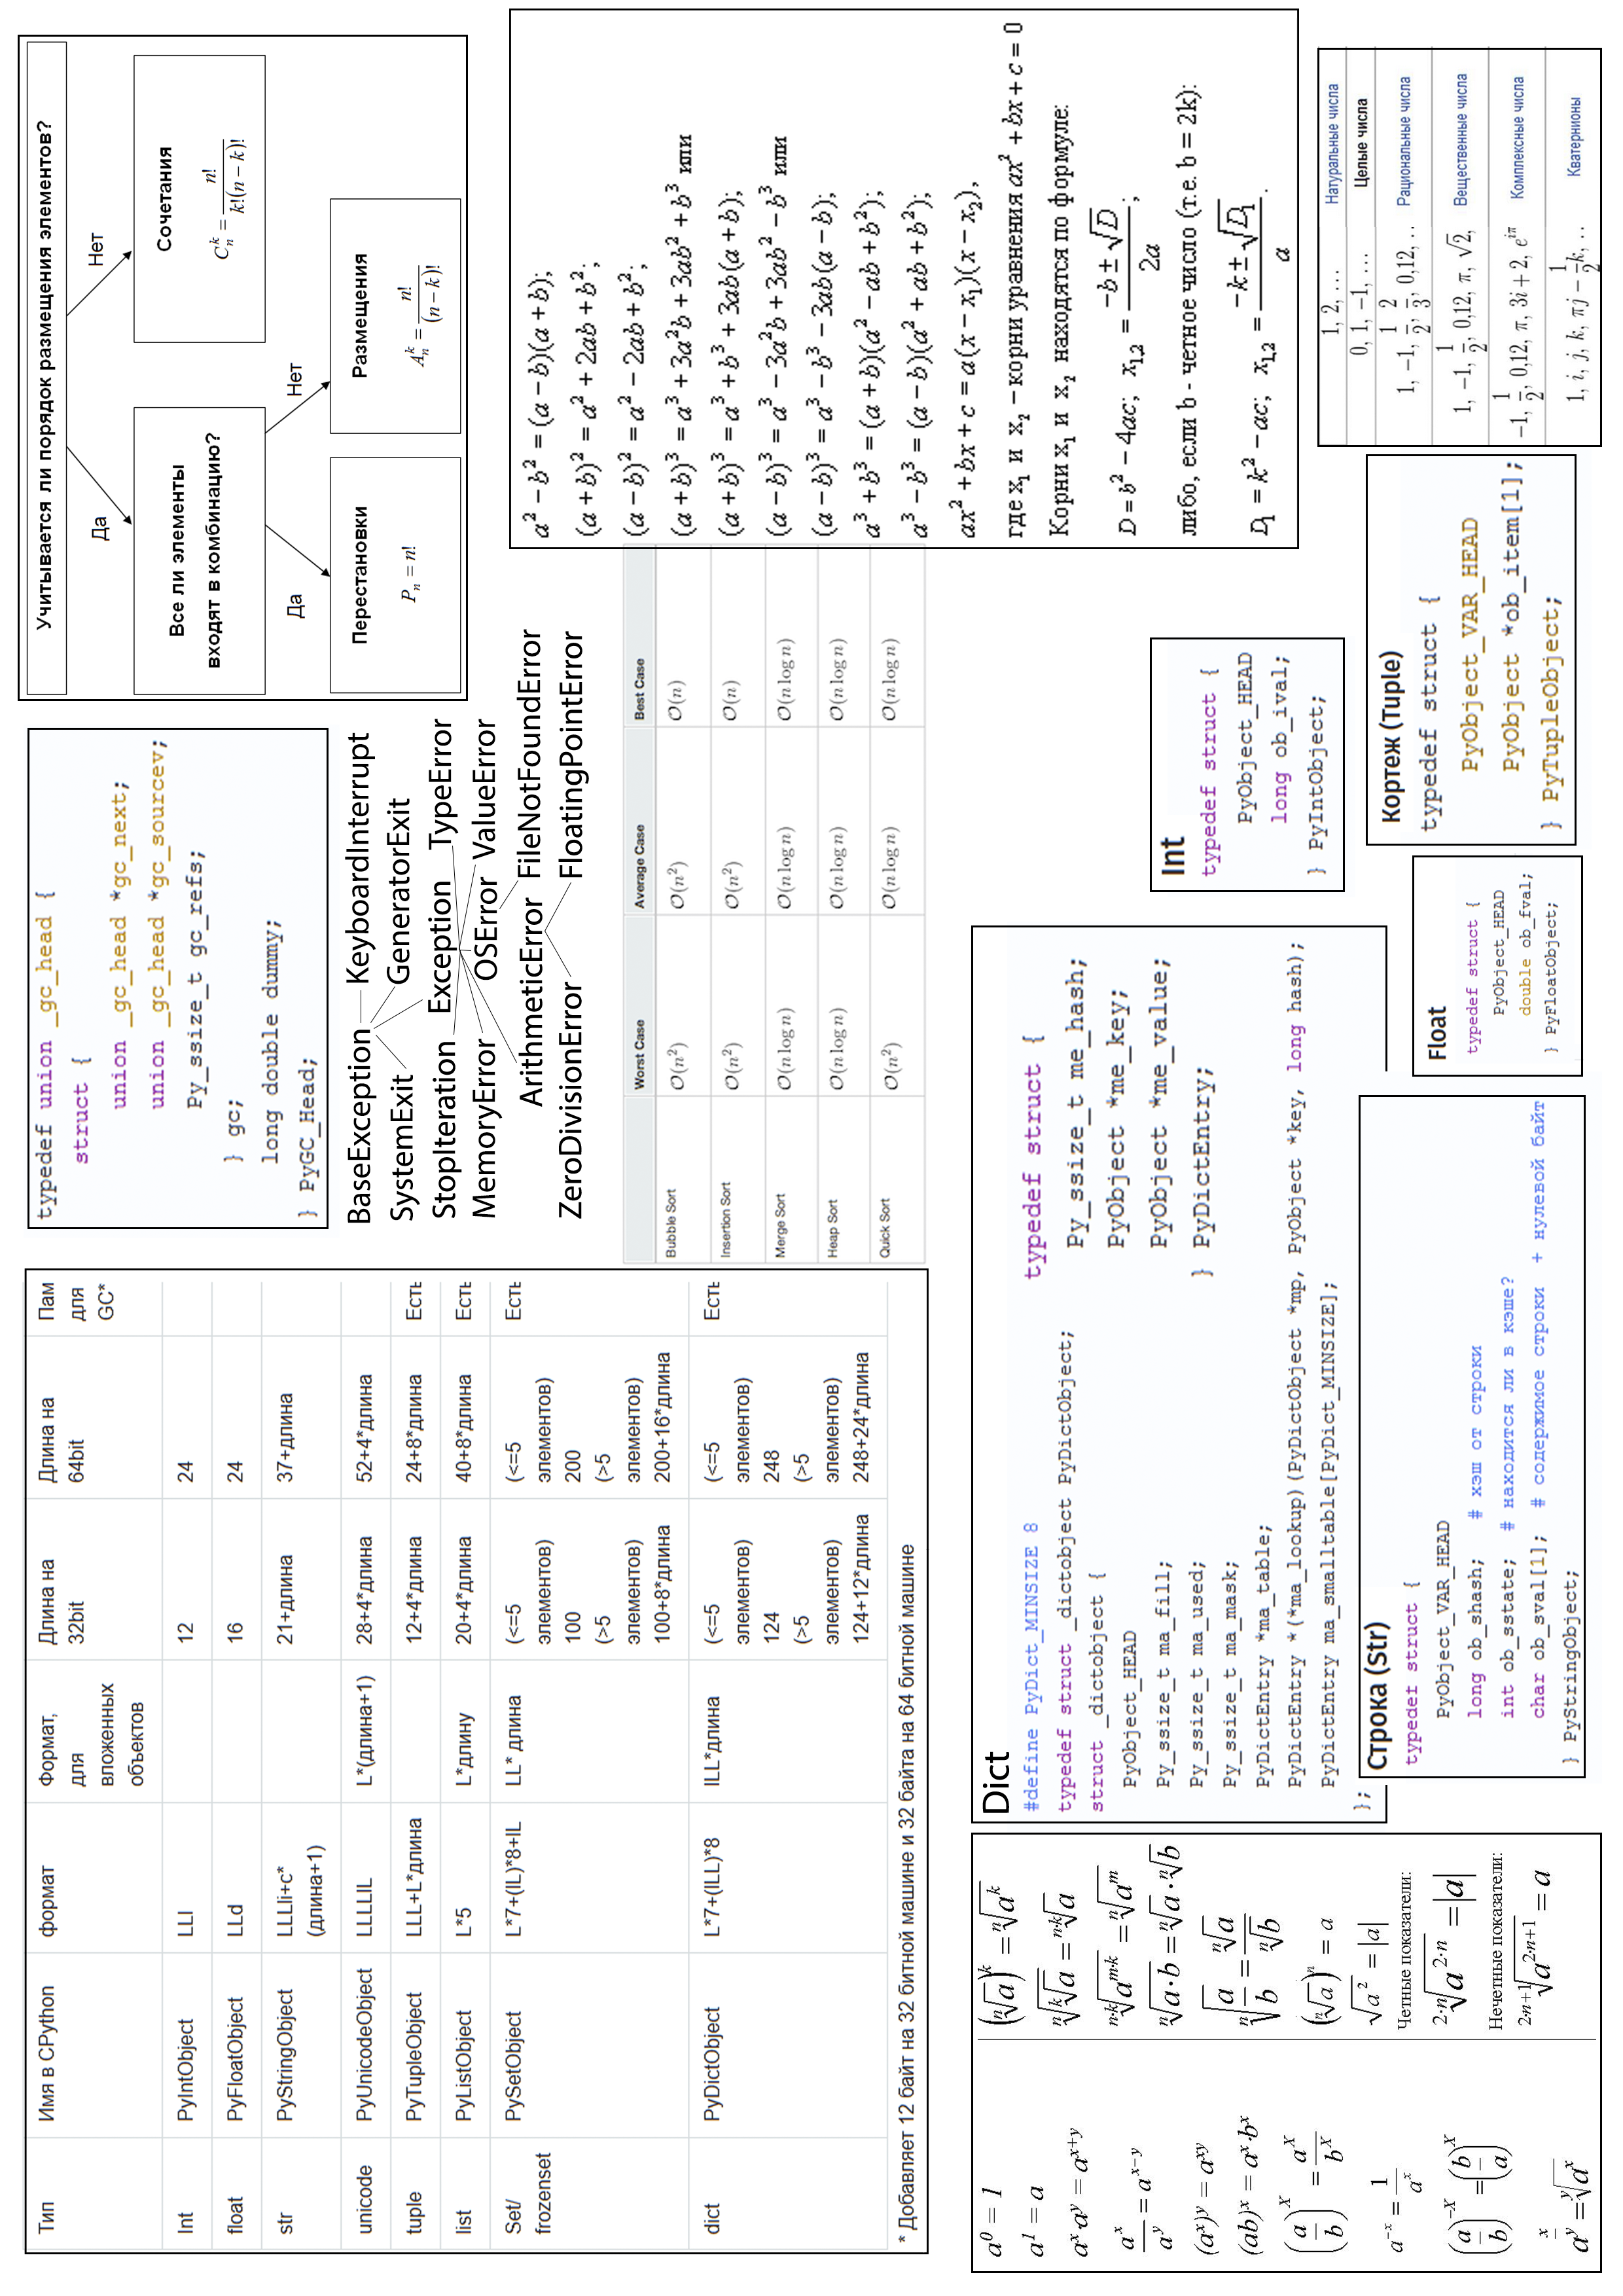
\includegraphics[width=\textwidth]{py_data_size.png}
\caption{Python usefull things}
\label{scheme}
\end{figure}

\section{Структуры базовых типов}

\section{GIL}

\subsection{Алгоритм работы}
\subsection{Эффективность переключения}

\section{Поколения сборщиков мусора}

\subsection{Алгоритм посчета ссылок}

\subsection{Отключение и ручной вызов GC2}

\chapter{Различные аспекты}

\section{Вызов в главной функции}
Что значит \pyth{if __name__=='__main__':}

Когда интерпретатор Python читает исходный файл, он исполняет весь найденный в нем код. Перед тем, как начать выполнять команды, он определяет несколько специальных переменных. Например, если интерпретатор запускает некоторый модуль (исходный файл) как основную программу, он присваивает специальной переменной \pyth{__name__} значение \pyth{"__main__"}. Если этот файл импортируется из другого модуля, переменной \pyth{__name__} будет присвоено имя этого модуля.

В случае с вашим сценарием, предположим, что код исполняется как основная функция, например:

\pyth{python threading_example.py}

После задания специальный переменных интерпретатор выполнит инструкцию import и загрузит указанные модули. Затем он проанализирует блок def, создаст объект-функцию и переменную под названием myfunction, которая будет указывать на этот объект.

Затем он прочтет инструкцию if, «поймёт», что \pyth{__name__} эквивалентен \pyth{"__main__"}, и выполнит указанный блок.

Одна из причин делать именно так – тот факт, что иногда вы пишете модуль (файл с расширением .py), предназначенный для непосредственного исполнения. Кроме того, он также может быть импортирован и использован из другого модуля. Производя подобную проверку, вы можете сделать так, что код будет исполняться только при условии, что данный модуль запущен как программа, и запретить исполнять его, если его хотят импортировать и использовать функции модуля отдельно.

Дополнительно см. \url{http://ibiblio.org/g2swap/byteofpython/read/module-name.html}.

\section{Импортирование модулей}
Что означает \pyth{threading_example} в данный момент импортируется из другого модуля?

Это означает, что кем-то в каком-либо файле .py (или в ходе интерактивной Python-сессии) используется выражение \pyth{import threading_example}. Противоположный этому случай – пользователь использует выражение \pyth{python threading_example.py} или \pyth{./threading_example.py}, и т. д.. В последнем случае, \pyth{threading_example.py} запущен как основная программа. В первом же случае он запущен как-то иначе (чтобы понять, ищите вызов вида \pyth{import threading_example}).

\section{Порядок вызова спец методов new, init, enter, exit, del}

Порядок вызова:

\begin{enumerate}
	\item \pyth{__new__()};
	\item \pyth{__init__()};
	\item \pyth{__enter__()}, если вызывается инструкция with;
	\item \pyth{__exit__()}, если вызывается инструкция with;
	\item \pyth{__del__()}
\end{enumerate}

\part{Реализация шаблонов (паттернов) проектирования}

\section{Сингелтон (Singleton)}

\linenumbers
\inputpython{singleton.py}{1}{100}
\nolinenumbers

\section{Adapter}

\section{Factory}

\section{Dependency}

\section{Injection}

\part{Общие задачи}

	\section{Вычисление факториала \label{tasks:fac}}
	Задача имеет множество решений. По этой причине реализуем хотя бы несколько с проверкой ответа из библиотеки python..
	
\linenumbers
\inputpython{factorials.py}{1}{100}
\nolinenumbers

	\section{Числа Фибоначчи \label{tasks:fib}}
	
	\section{Определение простых чисел \label{tasks:simple} }
	
\linenumbers
\inputpython{simple-nums.py}{1}{100}
\nolinenumbers
	
	\section{Найти наименьший общий делитель двух чисел (НОД)}
	\textbf{Алгоритм Евклида}:
	\begin{enumerate}
\item Большее число делим на меньшее.
\item Если делится без остатка, то меньшее число и есть НОД (следует выйти из цикла).
\item Если есть остаток, то большее число заменяем на остаток от деления.
\item Переходим к пункту 1.

	\end{enumerate}
	
	\section{Найти наибольшее общее кратное двух чисел (НОК)}
	
	\section{Работа с датами}
	\textbf{Задача:}
	
	Дана таблица в базе данных SQL состоящая из колонок: имя трудяги, дата устройства на работу, дата увольнения\dots необходимо выбрать всех работников которые:
	\begin{enumerate}
	\item отработали в текущем месяце больше 20 дней
	\item отработали за все время больше 30 дней
	\item уволились меньше чем через 60 дней
	\end{enumerate}
	
	\textbf{Решение:}
	
	
	
	\section{Шифр Цезаря}
Шифр Цезаря заключается в замене каждого символа входной строки на символ, находящийся на несколько позиций левее или правее его в алфавите.

Для всех символов сдвиг один и тот же. Сдвиг циклический, т.е. если к последнему символу алфавита применить единичный сдвиг, то он заменится на первый символ, и наоборот.

Напишите программу, которая шифрует текст шифром Цезаря.

Используемый алфавит − пробел и малые символы латинского алфавита: ' abcdefghijklmnopqrstuvwxyz'

\textbf{Формат ввода:}
На первой строке указывается используемый сдвиг шифрования: целое число. Положительное число соответствует сдвигу вправо. На второй строке указывается непустая фраза для шифрования. Ведущие и завершающие пробелы не учитывать.

\textbf{Формат вывода:}
Единственная строка, в которой записана фраза: Result: "..." , где вместо многоточия внутри кавычек записана зашифрованная последовательность.

\textbf{Примеры}

\begin{lstlisting}
Sample Input 1:
3
i am caesar
Sample Output 1:
Result: "lcdpcfdhvdu"
Sample Input 2:
-2
az
Sample Output 2:
Result: "zx"
Sample Input 3:
27
abc
Sample Output 3:
Result: "abc"
\end{lstlisting}

Решение:

\linenumbers
\inputpython{task1.py}{1}{100}
\nolinenumbers

\section{Парсинг лог файла}

\linenumbers
\inputpython{parse-log.py}{1}{100}
\nolinenumbers	

\section{Задача со столиками}

\subsection{Условие}

В вашем ресторане есть набор столов разных размеров: на каждом столе могут разместиться 2, 3, 4, 5 или 6 человек. Клиенты прибывают в одиночку или группами, до 6 человек. Клиенты в данной группе должны находиться вместе за одним столом, поэтому вы можете направить группу только к столу, который может вместить их всех. Если нет таблицы с необходимым количеством пустых стульев, группе приходится ждать в очереди.

После размещения группа не может изменить таблицу, т. Е. Вы не можете переместить группу из одной таблицы в другую, чтобы освободить место для новых клиентов.

Группы клиентов должны обслуживаться в порядке прибытия, за одним исключением: если на столе достаточно места для небольшой группы, прибывающей позже, вы можете разместить их перед более крупной группой (группами) в очереди. Например, если есть группа из шести человек, ожидающая стол на шесть мест, и есть группа из двух человек, которые стоят в очереди или прибывают, вы можете отправить их прямо к столу с двумя пустыми стульями.

Группы могут совместно использовать столы, однако если в то же время у вас есть пустой стол с необходимым количеством стульев и достаточным количеством пустых стульев за большим, вы всегда должны размещать своих клиентов за пустым столом, а не частично сидящими. , даже если пустая таблица больше, чем размер группы.

Конечно, система предполагает, что любая большая группа может устать от того, что меньшие группы приходят и опережают их столы, а затем решают уйти, что будет означать, что они покидают очередь без обслуживания.

Пожалуйста, заполните класс RestManager соответствующими структурами данных и реализуйте его конструктор и три открытых метода. Также рекомендуется изменить другие классы (чтобы мы могли их протестировать) и добавить новые методы по вашему желанию.

\subsection{Решение}





\part{Docker}

\chapter{Под копотом}

\section{Из каких базовых вещей состоят контейнеры: namespaces, cgroups}
Все инструменты контейнеризации — будь то Docker, LXC или systemd-nspawn,— основываются на двух подсистемах ядра Linux: namespaces и cgroups. 

\subsection{chroot}

Идеи, лежащие в основе механизма пространств имён, не новы. Ещё в 1979 году в UNIX был добавлен системный вызов chroot() — как раз с целью обеспечить изоляцию и предоставить разработчикам отдельную от основной системы площадку для тестирования. 

Название chroot представляет собой сокращение от change root, что дословно переводится как «изменить корень». С помощью системного вызова chroot() и соответствующей команды можно изменить корневой каталог. Программе, запущенной с изменённым корневым каталогом, будут доступны только файлы, находящиеся в этом каталоге. 

Вершиной этой иерархии является каталог /, он же root. Все остальные каталоги — usr, local, bin и другие, — связаны с ним.

С помощью chroot в систему можно добавить второй корневой каталог, который с точки зрения пользователя ничем не будет отличаться от первого. Файловую систему, в которой присутствует изменённый корневой каталог, можно схематично представить на рис. \ref{3}.

\begin{figure}[h!]
\centering
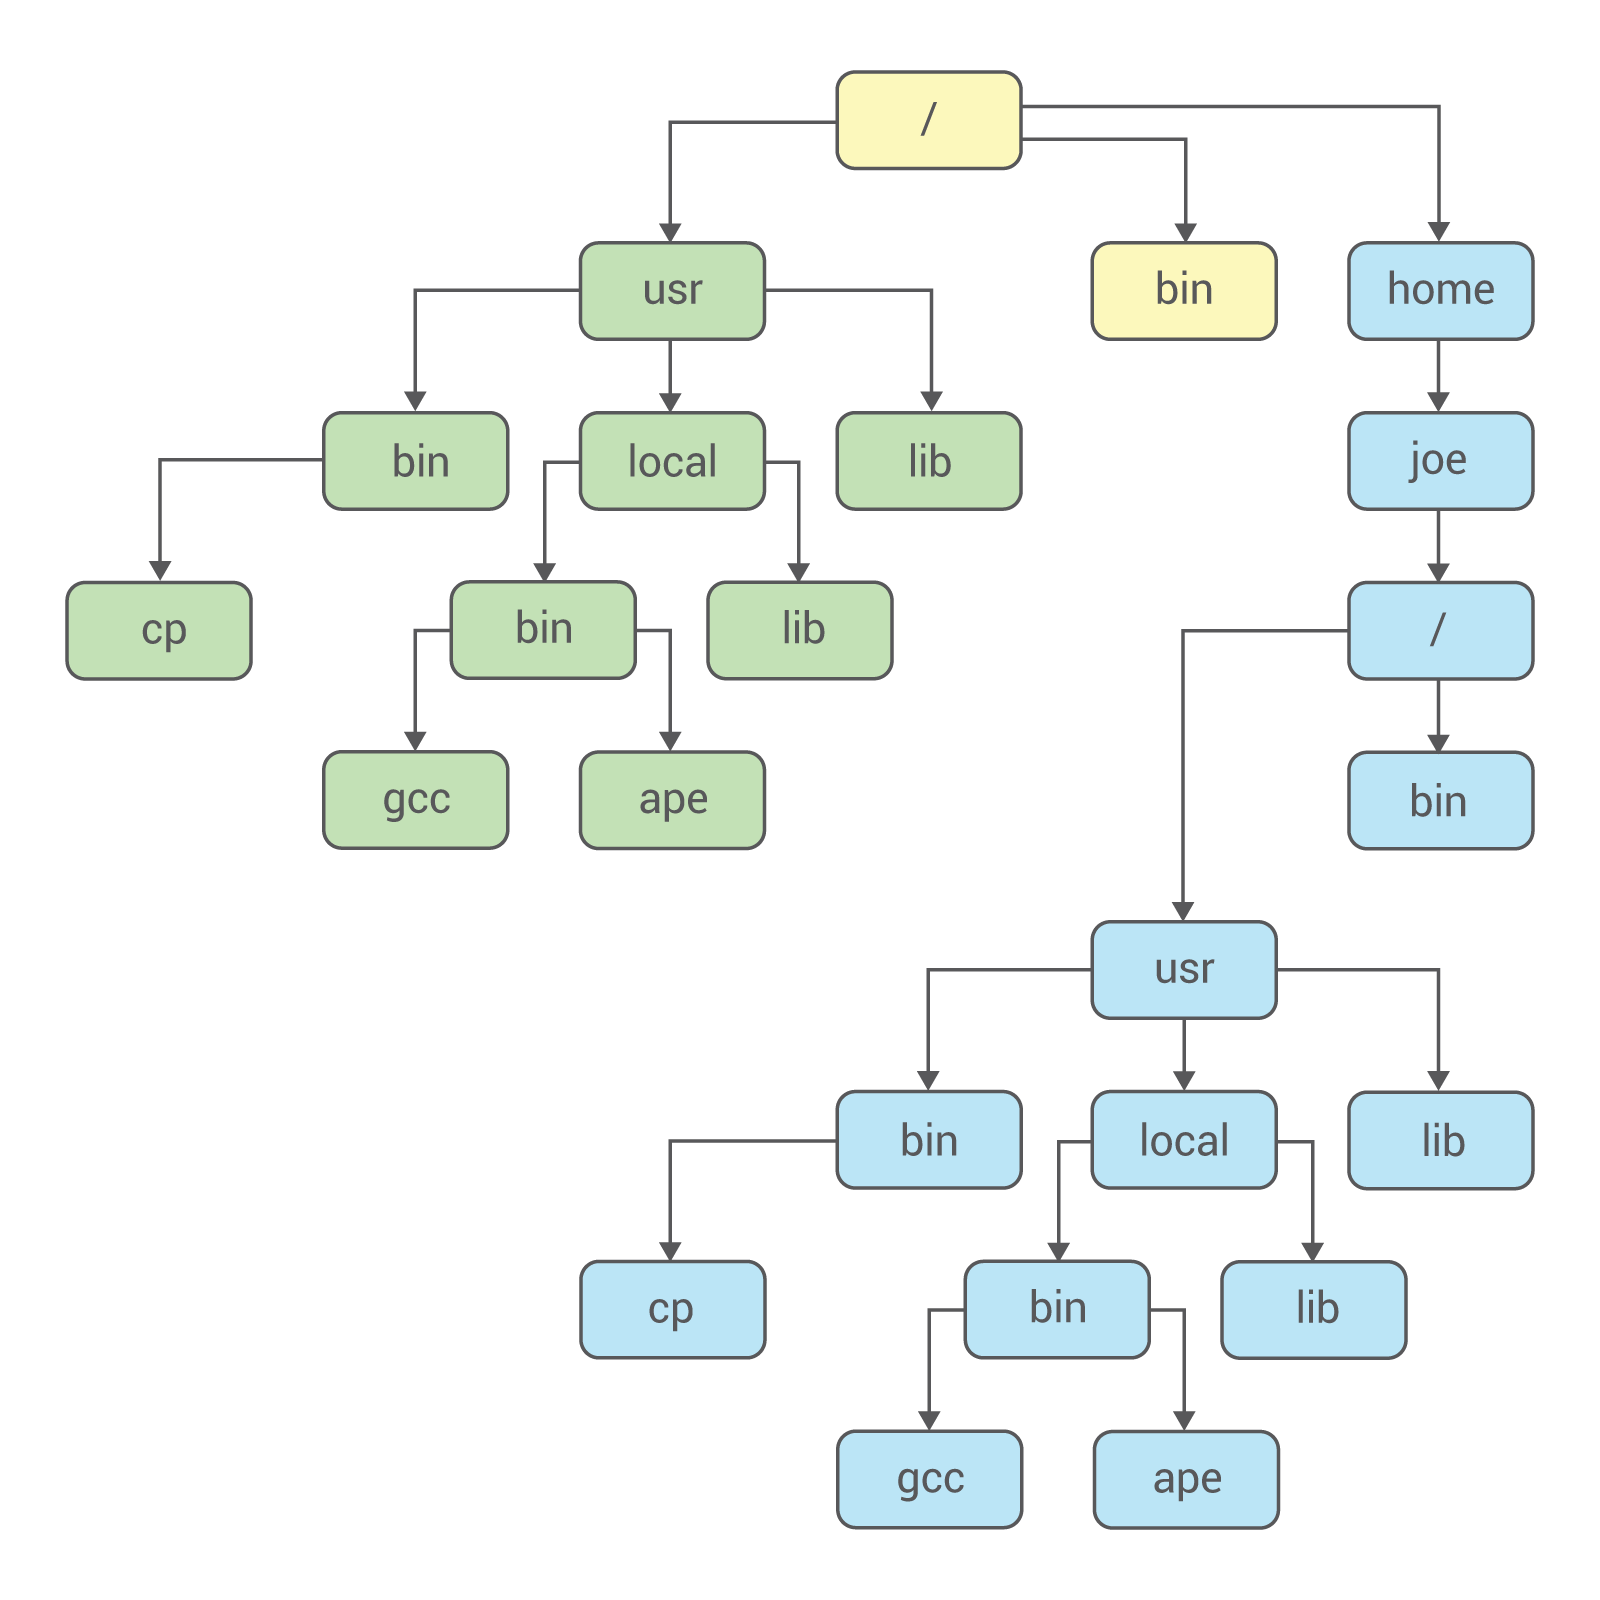
\includegraphics[width=0.9\textwidth]{img/chroot.png}
\caption{Представление файловой системы linux}
\label{chroot}
\end{figure}

\subsection{namespaces}

Пространство имён (англ. namespace) — это механизм ядра Linux, обеспечивающий изоляцию процессов друг от друга. Работа по его реализации была начата в версии ядра 2.4.19. На текущий момент в Linux поддерживается шесть типов пространств имён:

\begin{table}[]
\begin{tabular}{|l|l|}
\hline
Пространство имен & Что изолирует  \\ \hline
PID & PID процессов  \\ \hline
NETWORK & Сетевые устройства, стеки, порты... \\ \hline
USER & ID пользователей и групп \\ \hline
MOUNT & Точки монтирования \\ \hline
IPC & SystemV IPC, очереди сообщений POSIX \\ \hline
UTS & Имя хоста и доменное имя NIS \\ \hline
\end{tabular}
\end{table}

Неймспейсы изолируют друг от другая процессы таким образом, что процессы в одной группе не могут видеть ресурсы другой группы. Например, PID namespace предоставляет уникальные идентификаторы процессов в рамках группы. Внутри одной группы может быть процесс с pid 1 и внутри второй группы тоже может быть процесс с pid 1, хотя это два совершенно разных процесса, которые друг о другие ничего не знают. Притом, все процессы все также имеют уникальные id в рамках ОС. Просто, если смотреть на процессы из группы, то эти id отображаются в другие.

\subsubsection{PID: изоляция PID процессов}

При загрузке в Linux сначала запускается процесс с идентификационным номером (PID) 1. В дереве процессов он является корневым. Он запускает другие процессы и службы. Механизм namespaces позволяет создавать отдельное ответвление дерева процессов с собственным PID 1. Процесс, который создаёт такое ответвление, являются частью основного дерева, но его дочерний процесс уже будет корневым в новом дереве.

Процессы в новом дереве никак не взаимодействуют с родительским процессом и даже не «видят» его. В то же время процессам в основном дереве доступны все процессы дочернего дерева. Наглядно это показано на рис.

\begin{figure}[h!]
\centering
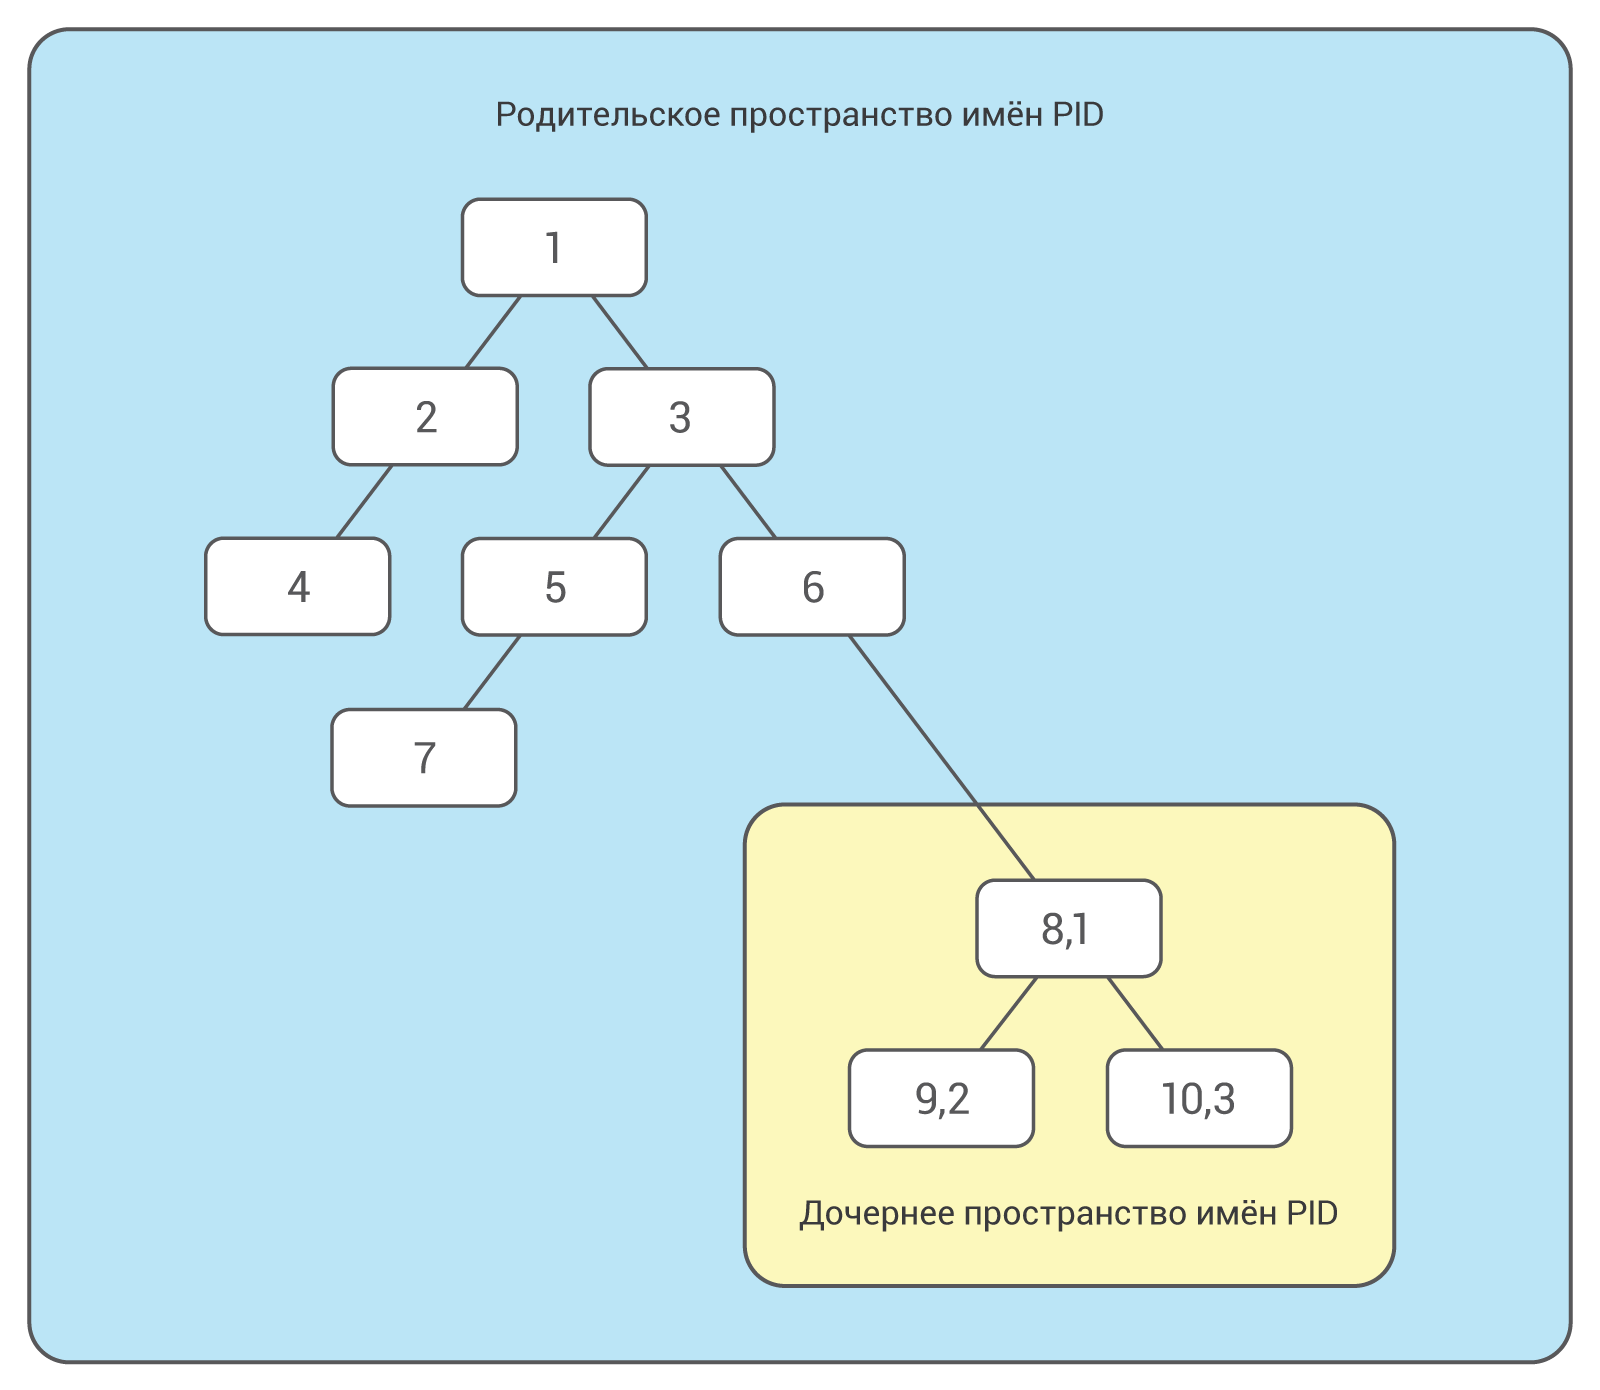
\includegraphics[width=0.9\textwidth]{img/pid.png}
\caption{Изоляция процессов}
\label{pid}
\end{figure}

\subsubsection{NET: изоляция сетей}

Благодаря пространству имён NET мы можем выделять для изолированных процессов собственные сeтевые интерфейсы. Даже loopback-интерфейс для каждого пространства имён будет отдельным.

Сетевые пространства имён можно создавать с помощью системного вызова clone() с флагом CLONE\_NEWNET. 

\subsubsection{MOUNT: изоляция файловой системы}

Об изоляции на уровне файловой системы мы уже упоминали выше, когда разбирали системный вызов chroot (). Мы отметили, что системный вызов chroot() не обеспечивает надёжной изоляции. С помощью же пространств имён MOUNT можно создавать полностью независимые файловые системы, ассоциируемые с различными процессами.

\subsection{cgroups (Control Groups)}

Позволяют организовывать процессы в группы и для каждой группы задавать лимиты. Например, лимиты на использование CPU, объем используемой памяти и дисковый ввод-вывод.

Механизм cgroups состоит из двух составных частей: ядра (cgroup core) и так называемых подсистем. В ядре версии 4.4.0.21 таких подсистем 12:

\begin{itemize}
\item blkio — устанавливает лимиты на чтение и запись с блочных устройств;
\item cpuacct — генерирует отчёты об использовании ресурсов процессора;
\item cpu — обеспечивает доступ процессов в рамках контрольной группы к CPU;
\item cpuset — распределяет задачи в рамках контрольной группы между процессорными ядрами;
\item devices — разрешает или блокирует доступ к устройствам;
\item freezer — приостанавливает и возобновляет выполнение задач в рамках контрольной группы
\item hugetlb — активирует поддержку больших страниц памяти для контрольных групп;
\item memory — управляет выделением памяти для групп процессов;
\item net\_cls — помечает сетевые пакеты специальным тэгом, что позволяет идентифицировать пакеты, порождаемые определённой задачей в рамках контрольной группы;
\item netprio — используется для динамической установки приоритетов по трафику;
\item pids — используется для ограничения количества процессов в рамках контрольной группы.
\end{itemize}

Каждая подсистема представляет собой директорию с управляющими файлами, в которых прописываются все настройки.  

\subsection{Отличия namespaces от cgroups}

\textbf{cgroup}: Контрольные группы предоставляют механизм для агрегирования или разбиения наборов задач и всех их будущих детей в иерархические группы со специализированным поведением.
\textbf{namespace}: обертывает глобальный системный ресурс в абстракции, которая заставляет его казаться процессам в пространстве имен, что у них есть свой отдельный экземпляр глобального ресурса.

\textbf{Вкратце}:

 cgroups = ограничивает, сколько вы можете использовать;
 namespaces = пределы того, что вы можете видеть (и, следовательно, использовать)

\section{Как docker прокидывает порт}

\chapter{Шпаргалка}

Полезная \href{https://docs.docker.com/engine/reference/builder/#usage}{ссылка} на документацию по основным операторам Dockerfile.

\subsection{ENV}

Пример использования в Dockerfile:
\begin{lstlisting}
ENV EDITOR 
\end{lstlisting}

\subsection{ARG}

Сборка с использованием аргументов, указать строку в Dockerfile:
\begin{lstlisting}
ARG UID
\end{lstlisting}

Аргументы по-умолчанию:
\begin{lstlisting}
ARG UID=1000
\end{lstlisting}

При сборке использовать параметр:
\begin{lstlisting}
docker build --build-arg UID=what_user .
\end{lstlisting}

\subsection{USER}

Специфицирует пользователя, под которым должен быть запущен образ. Мы можем указать имя пользователя или UID и группу или GID. Варианты использования команды:
\begin{lstlisting}
USER user
USER user:group
USER uid
USER uid:gid
USER user:gid
USER uid:group
\end{lstlisting}
Вы можете перегрузить эту команду, используя флаг -u при запуске контейнера. Если пользователь не указан, используется root по-умолчанию.

Пример конфигурирования пользователя при сборке, получая аргументом по-умолчанию UID: 
\begin{lstlisting}
ARG UID=1000
USER $UID
\end{lstlisting}

Сборка контейнера с заданием UID:
\begin{lstlisting}
docker build -t dockerfile-extended --build-arg UID=1001 .
\end{lstlisting}

\subsection{WORKDIR}

Создание и установка рабочей директории по-умолчанию:
\begin{lstlisting}
WORKDIR /home/stepik
\end{lstlisting}
Вы можете перегрузить рабочую директорию контейнера в рантайме с помощью флага -w.

\subsection{CMD и ENTRYPOINT}

The CMD instruction has three forms:
\begin{itemize}
\item CMD ["executable","param1","param2"] (exec form, this is the preferred form)
\item CMD ["param1","param2"] (as default parameters to ENTRYPOINT)
\item CMD command param1 param2 (shell form)
\end{itemize}

Это значит контейнеры собранные из этих файлов выводят одинаковую информацию:


\begin{itemize}
\item Без определения ENTRYPOINT:
\begin{lstlisting}
FROM ubuntu:latest
CMD ["printf", "Hello %s!\n", "World"]
\end{lstlisting}
\item С определением ENTRYPOINT:
\begin{lstlisting}
FROM ubuntu:latest
ENTRYPOINT ["printf"]
CMD ["Hello %s!\n", "World"]
\end{lstlisting}
\end{itemize}

\subsection{Передача параметров в контейнер}
Если быть точным, то это переопределение параметров запуска контейнера.
Если создать контейнер из файла:
\begin{lstlisting}
FROM ubuntu
ENTRYPOINT ["printf", "Hello %s!\n"]
CMD ["World"]
\end{lstlisting}
И запустить его командой:
\begin{lstlisting}
docker run --rm test
\end{lstlisting}
То вывод будет:
\begin{lstlisting}
Hello World!
\end{lstlisting}

Если изменить команду запуска:
\begin{lstlisting}
docker run --rm test John
\end{lstlisting}
То вывод будет:
\begin{lstlisting}
Hello John!
\end{lstlisting}


\section{ps}

\subsection{Просмотр работающих контейнеров}
\begin{lstlisting}
docker ps
\end{lstlisting}

\subsection{Просмотр всех контейнеров}
\begin{lstlisting}
docker ps -a
\end{lstlisting}

\section{run}

\subsection{Создание и запуск контейнера}
\begin{lstlisting}
docker run --rm -it --name new_name debian:latest bash
\end{lstlisting}

\begin{enumerate}
\item \textbf{--rm} - удалить контейнер после остановки.
\item \textbf{-it} - interactive tty, подключение к интерактивной консоли, в данном случае запуск bash.
\item \textbf{--name} - задаем имя контейнеру, в данном случае: new\_name.
\item \textbf{debian:latest} - обязательный параметр, образ от которого наследуемся.
\end{enumerate}

\subsection{Создание контейнера, который стартует при загрузке системы}
\begin{lstlisting}
docker run -d --restart=always debian:latest
\end{lstlisting}
\begin{enumerate}
\item \textbf{-d} - detach mode, если в контейнере есть "ожидающий или слушающий" процесс, то конейнер не завершится, пока его не попросить.
\item \textbf{--restart} - с параметром \textit{always} конейнер стартует сам.
\end{enumerate}

\subsection{Монтирование постоянного хранилища}
\begin{lstlisting}
docker run -d -v my_data:/etc/nginx/ debian:latest
\end{lstlisting}
Имя хранилища - \textit{my\_data}

\subsection{Монтирование постоянного папки хоста}
\begin{lstlisting}
docker run -d -v /var/log/nginx/:/tmp/logs/nginx/ debian:latest
\end{lstlisting}
\begin{itemize}
\item Имя папки хоста: /var/log/nginx/
\item Имя папки контейнера: /tmp/logs/nginx/
\end{itemize}


\subsection{Проброс порта}
\begin{lstlisting}
docker run -d -p 3344:80 debian:latest
\end{lstlisting}
\begin{itemize}
\item Номер внешнего порта хоста, доступный из сети: 3344
\item Номер порта контейнера доступный только из виртуальной сети docker: 80
\end{itemize}

\section{exec}
Подключение к уже работающему контейнеру:
\begin{lstlisting}
#Lets run bash from work container name 'worked_container':
docker exec -it worked_container bash
\end{lstlisting}

\section{volume}
\subsection{Создание хранилища для постоянных данных}
\begin{lstlisting}
docker volume create my_data
\end{lstlisting}

\subsection{Список осиротевших томов}
\begin{lstlisting}
docker volume ls -qf dangling=true
\end{lstlisting}


\section{network}
\section{commit}
Создание образа с изменением его точки входа:
\begin{lstlisting}
#Container create
docker run -it --name create-image-from-me ubuntu:14.04 /bin/true
#Lets change container and set new entry point:
docker commit --change='ENTRYPOINT ["/usr/bin/python3"]' create-image-from-me my-python:latest
#my-python:latest - new image name and tag
#Lets run new container from new image
docker run --rm -it my-python:latest
\end{lstlisting}



\section{build}

\subsection{Пример Dockerfile}

\lstinputlisting{Dockerfile1.txt}

\subsection{Сборка образа из Dockerfile}
\begin{lstlisting}
docker build -t myimage -f Dockerfile .
\end{lstlisting}
\begin{itemize}
\item \textbf{-t} - параметр определяющий имя нового образа.
\item \textit{-f} - задание Dockerfile не по-умолчанию, не обязательный параметр..
\item \textbf{.} - задание директории для сборки, в данном случае это будет текущая директория. Обязательный параметр.
\end{itemize}


\section{Полезные команды}
\subsection{Удалить все образы, не помеченные тегами}
\begin{lstlisting}
docker rmi $(docker images | grep '^<none>' | awk '{print $3}')
docker rmi $(docker images -f "dangling=true" -q)
\end{lstlisting}

\part{DevOps}

\section{Что такое load average}
Средняя загрузка — среднее значение загрузки системы за некоторый период времени, как правило, отображается в виде трёх значений, которые представляют собой усредненные величины за последние 1, 5 и 15 минут, чем ниже, тем лучше. В UNIX это среднее значение вычислительной работы, которую выполняет система.

Как правило, в UNIX-подобных системах вычисление средней загрузки происходит внутри ядра. Пользователи легко могут получить текущий показатель из командной оболочки, выполнив команду uptime: 

\begin{lstlisting}
14:34:03 up 10:43,  4 users,  load average: 0.06, 0.11, 0.09
\end{lstlisting}

Команды w и top показывают те же 3 значения средней нагрузки. В Linux они также могут быть получены путём прочтения файла \textbf{/proc/loadavg}. 

Nекстовый файл, предоставляемой пользователю виртуальной файловой системой /proc/, содержит 5 текстовых полей, разделенных пробелом. 
\begin{enumerate}
\item Первые три поля содержат значения, описанные выше, т.е. величины загрузки системы;
\item Четвертое поле состоит из двух чисел, разделенных слешем: число перед слешем показывает количество выполняемых в данный момент процессов; число после слеша показывает общее количество процессов в системе на данный момент;
\item Пятое поле показывает последний PID (идентификатор процесса), выделенных системой. 
\end{enumerate}

Чтобы понять, что такое загрузка системы следует обратиться к логике работы центрального процессора. Вне зависимости от того, мощный у вас процессор или слабый, многоядерный или нет, он выполняет некий программный код для некоторых процессов. Если процесс один, то вопросов нет, а вот когда их несколько? Надо как-то распределять ресурсы между ними и, желательно, равномерно, чтобы один процесс, дорвавшись до CPU, не оставил без вычислений другие.

Здесь можно провести аналогию, когда несколько игроков хотят поиграть на одной приставке. Что обычно делают в таких случаях? Договариваются о времени, скажем каждый играет по 15 минут, затем дает поиграть другому.

Процессор поступает аналогичным образом. Каждому нуждающемуся в вычислениях процессу выделяется некий промежуток времени, который зависит от типа процессора и системы, если говорить о современных процессорах Intel, то это значение обычно составляет 10 мс и называется тиком. Каждый тик процессорное время отдается какому-то одному процессу в порядке очереди, но если процесс имеет повышенный или пониженный приоритет, то он, соответственно получит большее или меньшее количество тиков.

Количество использованных тиков, в первом приближении, и представляет загрузку системы. В Linux для оценки загрузки используется интервал в 500 тиков (5 секунд), при этом учитываются как работающие процессы (использованные тики), так и ожидающие (которым не хватило тика, либо они не смогли его использовать, ожидая завершения иной операции).

Если мы используем все тики за указанный промежуток времени и у нас не будет ожидающих сводного тика процессов, то мы получим загрузку процессора на 100\% или load average (LA) равное 1.

\section{Что такое page cache?}

\section{Чем TCP отличается от UDP}

TCP гарантирует надежную и достоверную передачу(но это пожирает больше времени и траффика), как следствие у TCP существую понятия устаеновка соединения и разрыв соединения(обычно TCP используют при пересылки потоков информации, например FTP использует TCP), а UDP ничего не гарантирует(но это быстрее и меньше нагрузка сети), никаких соединений он не устанавливает, а шлет датаграммы(или как чаще пишут дейтаграммы) — законченные сообщения, причем небольшой длины, которые могут приходить на удаленный хост не в том порядке, в котором отправлялись, следовательно посредством UDP лучше не реализовывать передачу потоков информации(обычно по UDP посылаются сообщения, запросы и т.п.). Правда эффект с перемешиванием датаграмм в маленьких локальных сетях, в принципе, не происходит, да и потери при передаче обычно отсутствуют, тогда UDP используют для передачи потоковой информации(многие сетевые игры так делают.

\section{Устройство файловой системы}

\section{Что такое SWAP}
Если ваш компьютер пытается запустить программу, которая требует больше оперативной памяти, чем доступно, большинство современных операционных систем, для решения этой задачи, используют технологию swapping (подкачка). Суть этой технологии заключается в том, что некоторый объем данных (который не помещается в оперативную память) временно хранится на жестком диске, в то время как другая часть данных обрабатывается. В этой статье мы рассмотрим несколько вариантов управления своп-разделами в Linux для повышения производительности вашей системы.

В ОС Linux оперативная память (ОЗУ, RAM, random access memory) делится на разделы, называемые страницами (pages). Swapping (подкачка, своппинг) – это процесс во время которого страницы памяти копируются на специально сконфигурированный для этого раздел диска, называемый swap space (раздел подкачки, может быть как и файлом, так и разделом жесткого диска), для освобождения ОЗУ. Совокупные размеры физической памяти и раздела подкачки – это объем имеющийся виртуальной памяти.

Своппинг необходим по следующим причинам. Во-первых, когда системе необходимо больше памяти (т.е. приложение или процесс запрашивает у системы больше памяти) чем сейчас свободно в ОЗУ, ядро разгружает (откачивает) наименее используемые страницы и освобожденную память выделяет текущему приложению или процессу. А во-вторых, значительное количество страниц используемых программами на стадии запуска, используются только при инициализации и никогда более. Соответственно система может засвапить эти страницы, тем самым освобождая (разгружая) ОЗУ.

Тем не менее у своппинга есть и недостатки. По сравнению с ОЗУ, работа с жестким диском осуществляется на много медленнее. Для оценки временных затрат на чтение/запись в ОЗУ используются наносекунды, в то время как для жесткого диска используются миллисекунды, т.е. одни и теже операции на жестком диске занимают в десятки тысяч больше времени чем в ОЗУ. Следовательно чем больше страниц спаппится, тем медленнее работает ваша система. Иногда могут возникать такие проблемы, когда страница откачивается из ОЗУ, и через очень короткий промежуток времени закачивается обратно, и т.д., это приводит к сильному затормаживанию вашей системы. В таких ситуациях выход один – увеличить объем ОЗУ.

В Linux есть две формы своппа: раздел подкачки и файл подкачки. Раздел подкачки – это отдельный раздел на жестком диске, используемый только для своппинга, никакие другие файлы не могут там располагаться. Файл подкачки – это специальный файл в файловой системе.

\section{Устройство сетевого стека?}

\section{Можно ли забирать пакеты напрямую из сетевой карты?}

\chapter{Диски}

\section{Что такое trim? Continuous and periodic?}
\section{Что такое механизм wear leveling?} 
\section{Что такое over-provisioning?}
\section{Что такое garbage collector?}
\subsection{Какие планировщики есть? noop, deadline, cfq, bfq}
\subsection{Что такое разыменовывание символической ссылки?}
\subsection{Уровни Raid?}

\chapter{Сети}

\section{Модель OSI и стек TCP/IP}

Модель OSI состоит из 7 уровней рис. \ref{fig1} и \ref{fig2}:
\begin{enumerate}
\item Физический;
\item Канальный;
\item Сетевой;
\item Транспортный;
\item Сессионный;
\item Представления;
\item Прикладной;
\end{enumerate}

\begin{figure}[h!]
\centering
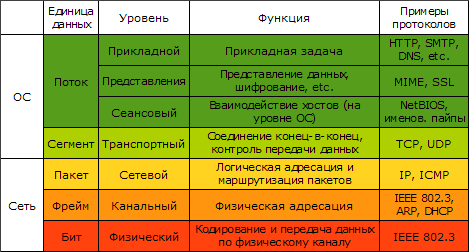
\includegraphics[width=0.8\textwidth]{img/exampleosi.png}
\caption{Описание модели OSI}
\label{fig1}
\end{figure}

Стек TCP/IP состоит из 4 слоев рис. \ref{fig2}:
\begin{enumerate}
\item Сетевой;
\item Интернета;
\item Транспортный;
\item Приложения;
\end{enumerate}

\begin{figure}[h!]
\centering
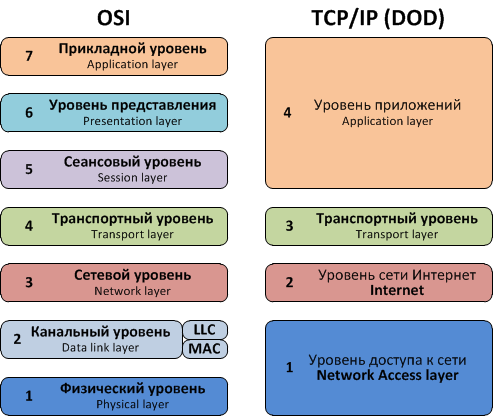
\includegraphics[width=0.8\textwidth]{img/ositcp.png}
\caption{Модель OSI и стек TCP/IP}
\label{fig2}
\end{figure}

\section{Отличия unicast anycast}

\begin{figure}[h!]
\centering
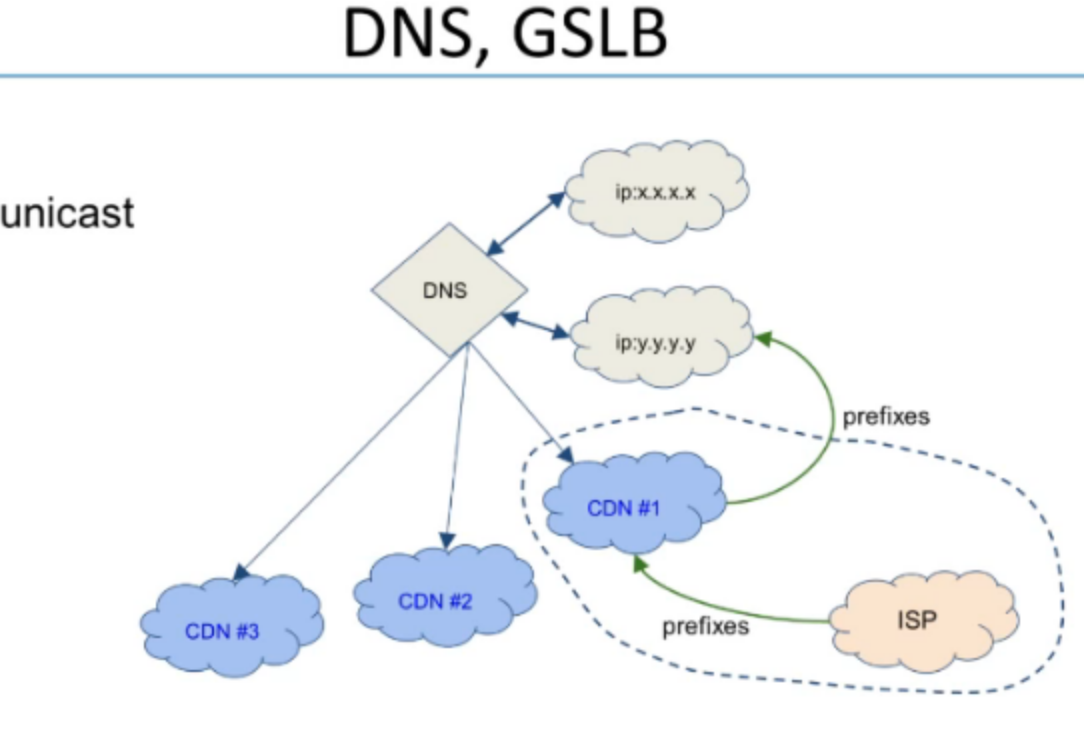
\includegraphics[width=0.8\textwidth]{img/unicast.png}
\caption{unicast}
\label{unicast}
\end{figure}

\section{Что такое CDN}

\section{Защита от SYN DDOS, Slow get/post, gzip bomb}

\section{Как избежать полного рукопажатия при tls?}

\section{Что такое BGP?}

\section{http 2?}

\section{websockets}

\begin{figure}[h!]
\centering
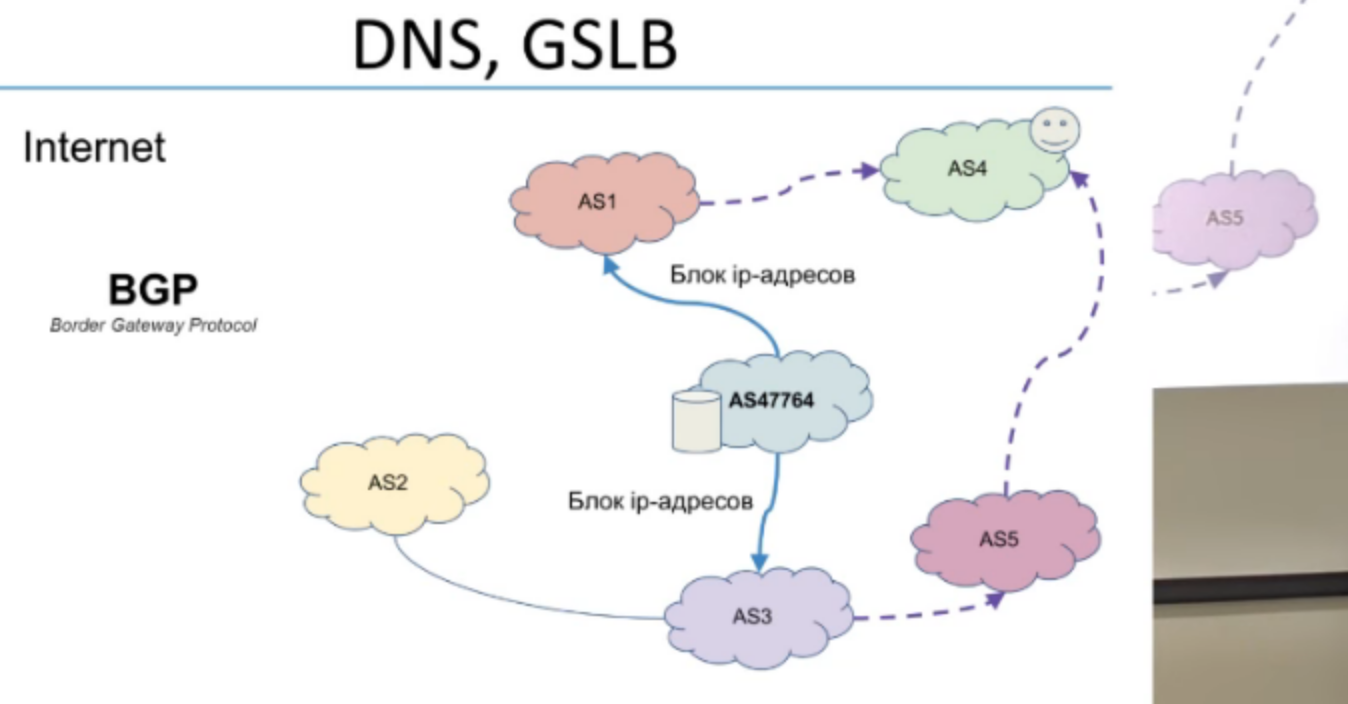
\includegraphics[width=0.8\textwidth]{img/BGP.png}
\caption{BGP}
\label{BGP}
\end{figure}

\chapter{Общие вопросы}

\section{Что такое DevOps}

DevOps (акроним от англ. development и operations) — это методология разработки ПО, сфокусированная на предельно активном взаимодействии и интеграции в одной упряжке программистов, тестировщиков и админов, синхронизировано обслуживающих общий для них сервис/продукт. Главная цель этого — создание единого цикла взаимозависимости разработки, эксплуатации и деплоя программного обеспечения, дабы в конечном счете помогать организациям (сервисам, стартапам) быстрее и безболезненней создавать и обновлять их программные продукты и сервисы, эксплуатируемые в режиме реального времени или «в продакшене».	

\section{Что такое Agile}
Agile — это не методология, а собирательное название различных методик и подходов к управлению, которые:

\begin{enumerate}
\item Фокусируют команду на нуждах и целях клиентов.
\item Упрощают оргструктуру и процессы.
\item Предлагают работу короткими циклами.
\item Активно используют обратную связь.
\item Предполагают повышение полномочий сотрудников.
\item Имеют в своей основе гуманистический подход.
\item Не являются конечным состоянием, а, скорее, образом мышления и жизни.
\end{enumerate}

\section{Что такое Kanban}

Канбан — это способ управления работой в духе Аджайла. Он содержит всего шесть правил и предлагает эволюционный переход от привычного образа мышления к аджайловому. Аджайл-коучи часто сравнивают Канбан с водой — он обтекает структуру и иерархию компании и медленно начинает их менять. Как вода точит камни, так Канбан меняет образ мышления.

\begin{enumerate}
\item Визуализируйте
\item Ограничивайте
\item Контролируйте
\item Договоритесь
\item Анализируйте
\item Экспериментируйте
\end{enumerate}


 \section{Типы балансировки, L3, L4, L7}
Распределение нагрузки по нескольким инстансам приложения.

\begin{figure}[h!]
\centering
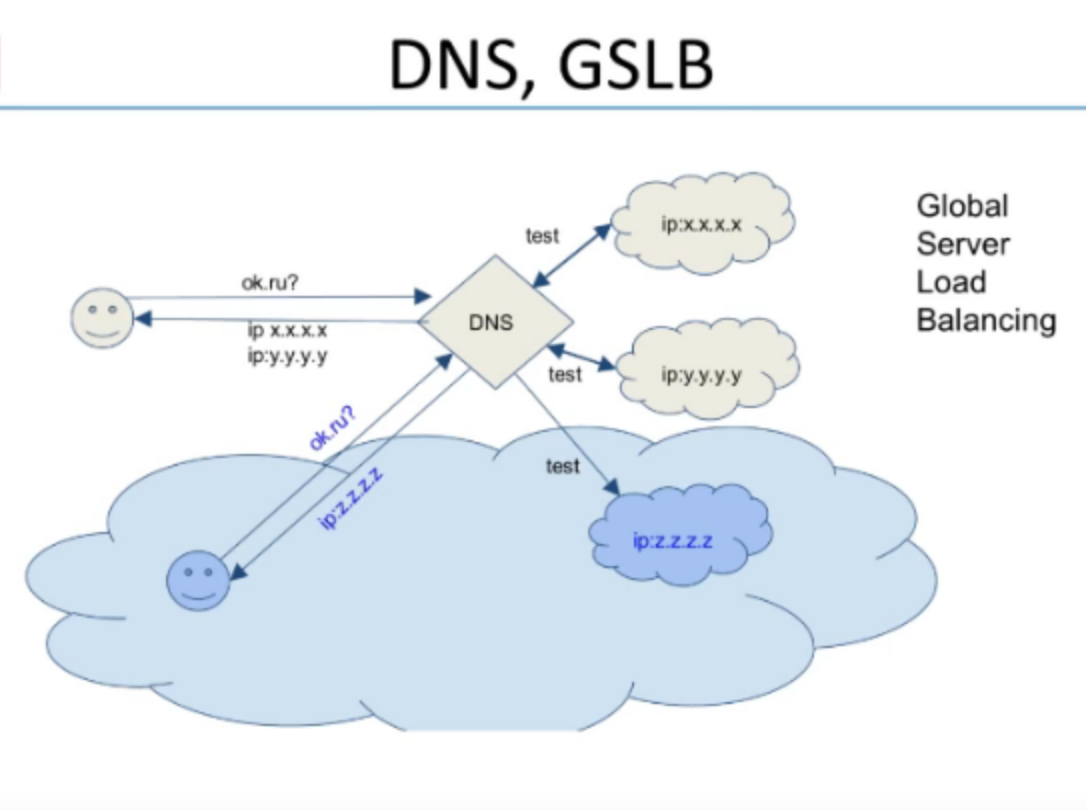
\includegraphics[width=0.8\textwidth]{img/balansing.png}
\caption{BGP}
\label{balansing}
\end{figure}
 
 \subsection{DNS Round Robin}
 Самый простой метод балансировки — это использование алгоритма DNS Round Robin. Суть его в том, что мы создаем несколько DNS-записей типа А для записи нашего домена на DNS-сервере. DNS-сервер выдает наши записи типа А в чередующемся циклическом порядке.
 
\subsection{Балансировка на втором уровне стека протоколов}     
 Следующий метод балансировки — это балансировка на втором уровне стека протоколов. Здесь можно выделить два варианта: балансировка с использованием отдельного выделенного балансировщика и без.

В обоих случаях мы берем некоторый IP-адрес нашего сервиса. Его мы устанавливаем для всех наших серверов либо на OBEC, либо на другой специализированный интерфейс. Делается это для того, чтобы данные серверы могли принимать соединения на этот IP-адрес и отвечать с него, но не отвечали бы на ARP-запросы, относящиеся к этому адресу.

Как работает такая балансировка? На балансировщик, имеющий этот IP-адрес и отвечающий на ARP, приходит, допустим, первый пакет соединения. Мы определяем, что он первый. Нужным алгоритмом отправляем его на интересующий нас сервер, меняя MAC-адрес на место назначения (англ. destination). Записываем его в некоторую таблицу соединений.

\subsection{Метод балансировки на третьем уровне}
Метод балансировки на третьем уровне стека протоколов, то есть на уровне протокола IP. В нем мы назначаем балансировщику тот же IP-адрес сервиса. Когда идет обращение на него, мы применяем так называемый Destination NAT, то есть подменяем IP-адрес назначения в пакете: IP-адреса текущего сервера меняется на выбранный по нужному алгоритму IP-адрес сервера, который будет обрабатывать запрос.

Отличие этого метода от предыдущего заключается в том, что мы модифицируем заголовки третьего уровня. Поэтому для ответов нам их также нужно модифицировать, провести обратную операцию замены. IP-адрес отправителя нужно поменять с IP-адреса сервера, который обрабатывает запрос, на IP-адрес сервиса, который используется на балансировщике.

\subsection{Метод проксирования}

Есть некоторый прокси-сервер, на котором используется IP-адрес нашего сервиса, он получает запрос, при необходимости что-то делает с ним и перенаправляет его уже от себя нужному серверу.

Этот метод для сервера уже не прозрачен, поскольку он видит, что к нему обращается наш прокси. Для этого внутри протокола высокого уровня мы должны каким-то образом передать сведения о том, какой же клиент к нам обращается. Для протокола HTTP мы можем добавлять заголовок X-Real-IP с IP-адресом клиента.

\subsection{Балансировка с помощью редиректа}
Есть некоторый балансировщик, который при обращении к нашему сервису (например, http://site.com) дает клиенту редирект на конкретный сервер (например, http://server2.site.com). В случае HTTP это будет выглядеть как "HTTP redirect 302", по-моему, код редиректа будет выглядеть как "временно перемещено" (англ. moved temporary).

\subsection{Балансировка L4}

\begin{figure}[h!]
\centering
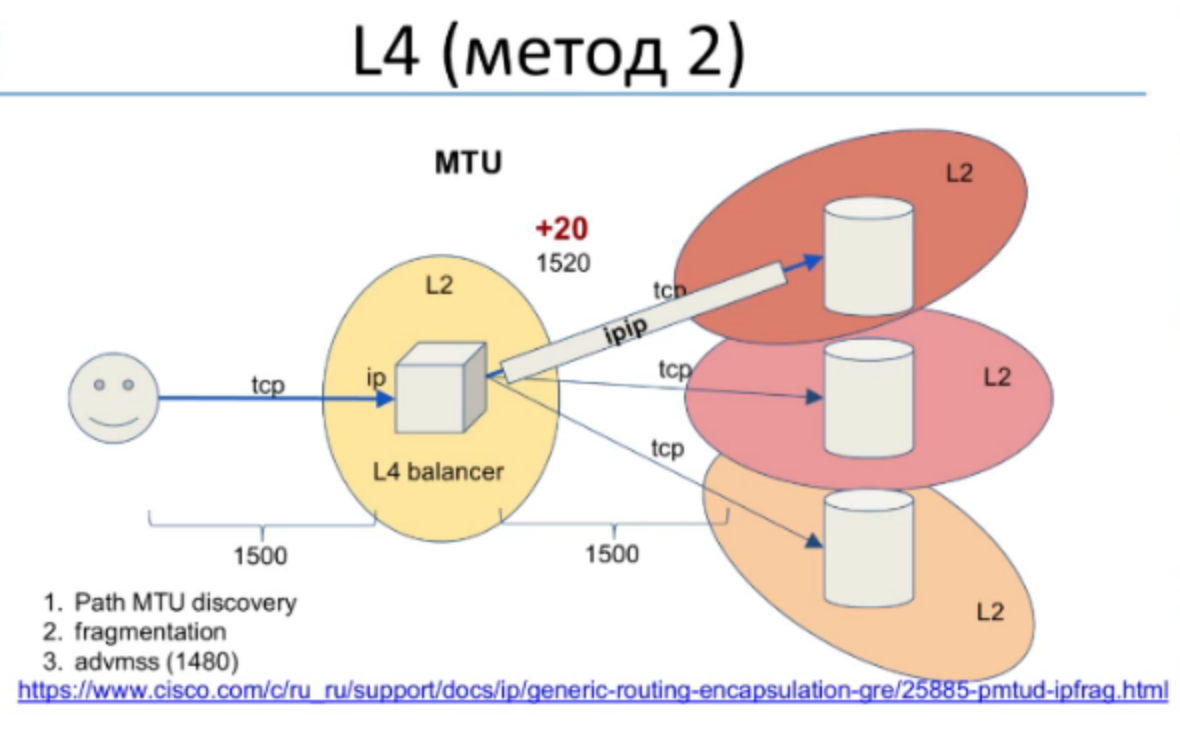
\includegraphics[width=0.8\textwidth]{img/L41.png}
\caption{Балансировка L4}
\label{L41}
\end{figure}


\begin{figure}[h!]
\centering
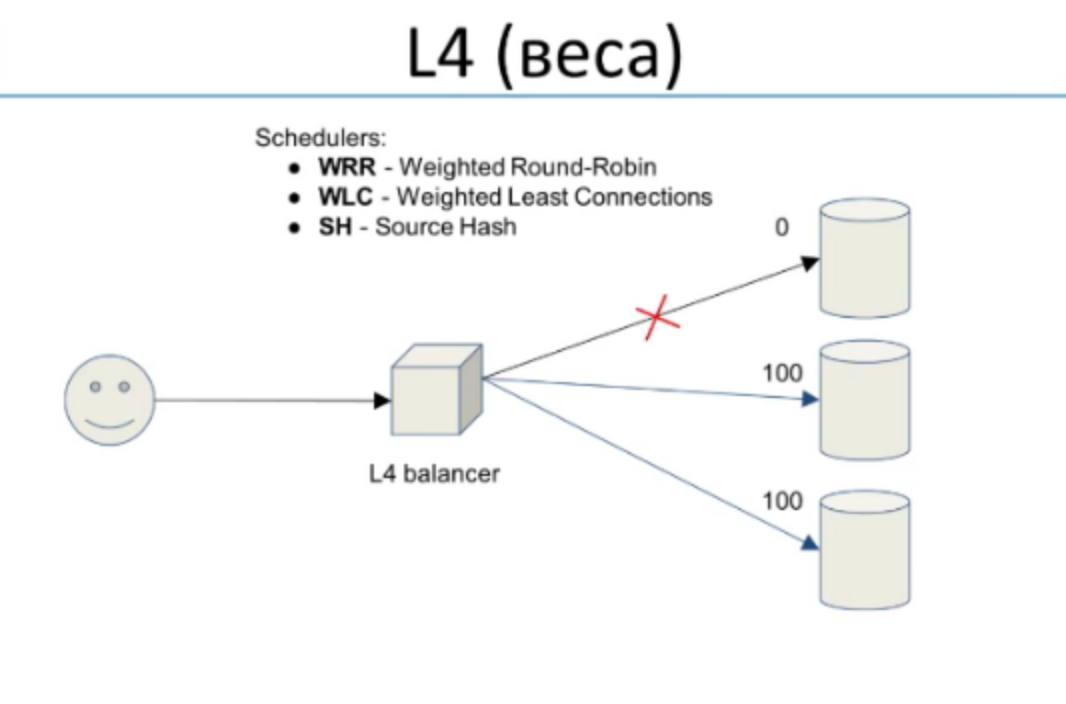
\includegraphics[width=0.8\textwidth]{img/L4-weights1.png}
\caption{Балансировка L4 c весами}
\label{L4w1}
\end{figure}


\begin{figure}[h!]
\centering
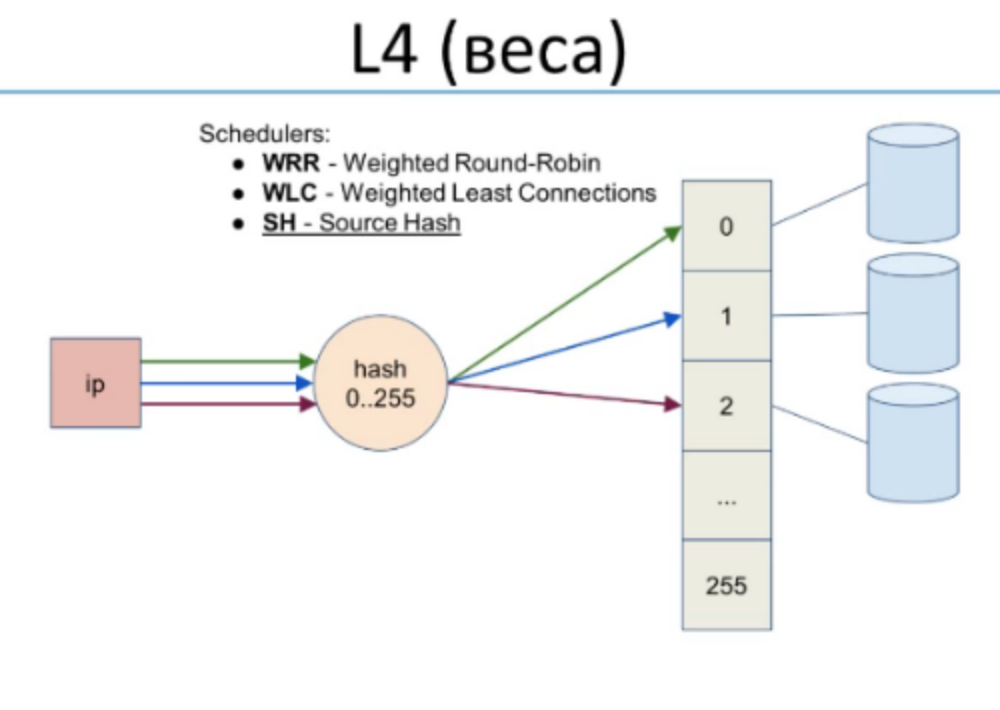
\includegraphics[width=0.8\textwidth]{img/L4-weights2.png}
\caption{Балансировка L4 с весами}
\label{L4w2}
\end{figure}

\section{Сине-зеленый деплой (blue-green deploy)}

Одна из задач автоматизации деплоя — переход из одного состояния в другое внутри себя же, с переводом софта из финальной стадии тестирования в действующий продакшен. Обычно это нужно сделать быстро, чтобы минимизировать время простоя. При \textbf{сине-зеленом подходе} у вас есть два продакшена, насколько возможно идентичных. В любое время один из них, допустим синий, активен. При подготовке новой версии софта, вы делаете финальное тестирование в зелёном продакшене. Вы убеждаетесь, что программа в этом продакшене работает и настраиваете роутер так, чтобы все входящие запросы шли в зелёную операционную среду — синяя в режиме ожидания.

\section{Какая разница между Continuous Delivery, Continuous Deployment и Continuous Integration}

\subsection{Continuous delivery (непрерывная доставка)}

В большинстве случаев непрерывная доставка — это серия практик, направленных на то, чтобы обновления программного обеспечения происходили практически постоянно. Данные методы гарантируют быстрое развёртывание на продакшене не меняя существующий функционал. Непрерывная доставка осуществима благодаря различным оптимизациям на ранних этапах процесса разработки.

Разработчик, сделав какую-либо фичу, отправляет её QA-инженерам для тестирования. Тестировщикам легче досконально оттестировать небольшой новый функционал и написать к нему тест-кейсы. Как только все проверки – прошли, новая фича попадает на дальнейшее тестирование авто-тестами и потом уже в релизный брэнч в системе контроля версий.


\subsection{Continuous deployment(непрерывное развёртываение)}

Continuous deployment часто путают с continuous delivery, хотя между ними существуют чёткие различия, которые следует знать и понимать.

Как выше было уже сказано непрерывная доставка обеспечивает постоянный выпуск обновлений пользователям. А непрерывное развёртывание отвечает за то, чтобы весь новый функционал после тестирования сразу же попал в основную программу без ручного вмешательства инженеров DevOps.

Тот же Docker создан для неприрывного развёртывания. DevOps инженеры могут обновлять контейнеры и разворачивать их сразу на продакшене в автоматическом режиме. Такой процесс является ключом к непрерывной доставке, т.к. весь процесс может занять всего лишь несколько минут.

Не всегда непрерывное развёртывание имеет смысл. Использование фича-тоглинга сводит на нет все преимущества. Всегда надо исходить из потребностей бизнеса и процессов внедрения нового функционала.

\subsection{Continuous integration (непрерывная интеграция)}

Непрерывная интеграция является ключевым компонентом практики Agile Development. Основой данной практики является постоянное попадание кода в центральный репозиторий после успешного запуска тестов. Основные цели continuous integration – поиск и устранение потенциальных проблем как можно быстрее, улучшение качества ПО и сокращение время для выпуска обновлений.

До того, как непрерывная интеграция стала широко распространённой, разработчики обычно работали изолировано, а только по окончанию работы объедениняли свои наработки. Порой это был очень трудоёмкий и длительный процесс.

При непрерывной интеграции разработчики часто заливают свои изменения в центральный репозиторий, выполняя до этого unit – тесты. Затем система контроля версий автоматически проверяет код на возможно безопасной интеграции с существующим в репозитории. При этом идёт постоянное поступление кода, что облегчает тестирование и сводит к минимуму возможные риски.

\begin{figure}[h!]
\centering
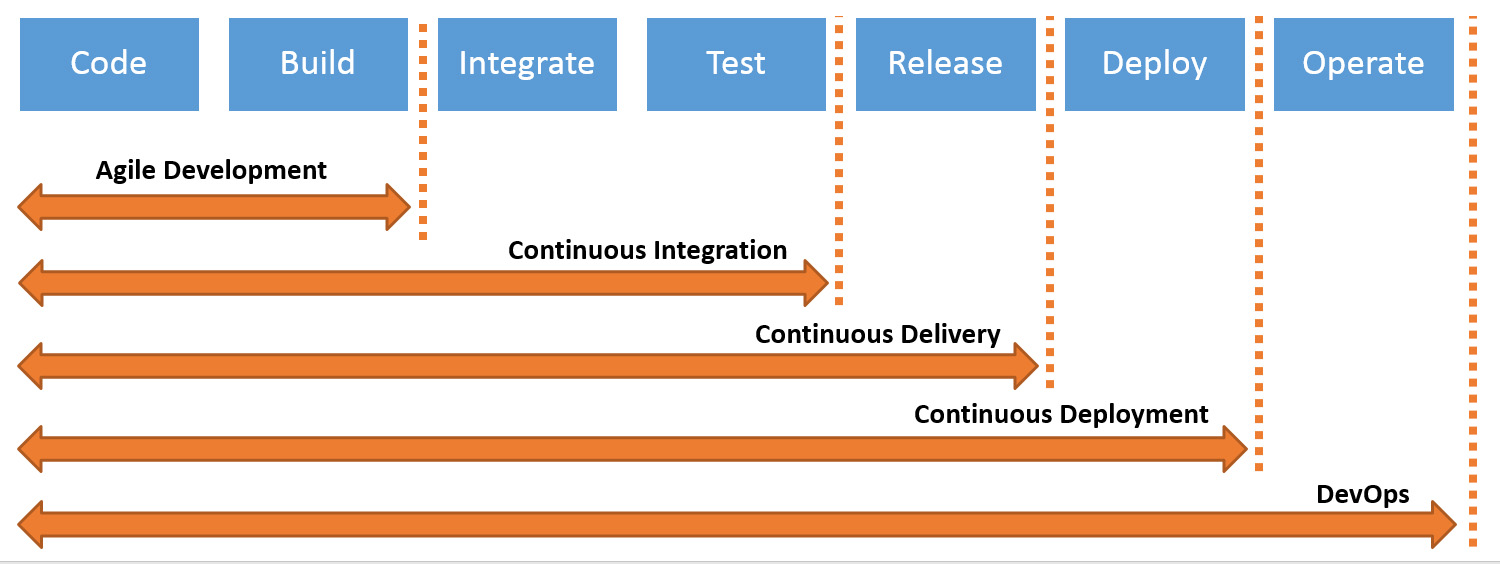
\includegraphics[width=0.9\textwidth]{img/ci-vs-cd-devops-difference.jpg}
\caption{Сравнение CI CD}
\label{fig5}
\end{figure}

\section{Как в access логе посмотреть самые активные ip за сутки}

\begin{lstlisting}
awk '{print $1, $9}' gitlab_access.log | uniq -c | sort -nk1 -r
\end{lstlisting}

\section{Системы управления конфигурациями Ansible/Puppet/Chef}
\section{CI системы Jenkins/TeamCity}
\section{Cтеком Hashicorp (Vault, Consul, Nomad, Teпaform}
\textbf{Vault} - хранилище секретов.

\textbf{Consul} предназначен для service discovery, как и, например, etcd или ZooKeeper. Но далеко не всем известно, что помимо service discovery также Consul имеет огромное количество других возможностей, например, встроенный мониторинг сервисов, распределенные локи, и другие. 
\section{Стек ELK (elasticsearch, logstash, kibana)}
\subsection{logstash}
logstash – это утилита для сборки, фильтрации и последующего перенаправления в конечное хранилище данных. Вы могли слышать о fluentd – logstash решает ту же самую задачу, но написан на jruby и чуть более лучше дружит с elasticsearch.
\subsection{elasticsearch}
Изначально, elasticsearch – это решение для полнотекстового поиска, построенное поверх Apache Lucene, но с дополнительными удобствами, типа лёгкого масштабирования, репликации и прочих радостей, которые сделали elasticsearch очень удобным и хорошим решением для высоконагруженных проектов с большими объёмами данных.
\subsection{kibana}
И вот у нас есть logstash, который собирает и обрабатывает данные со всех ваших тысяч серверов и elasticsearch, который изо всех сил эти данные хранит и позволяет искать по ним. Чего не хватает? Верно, не хватает Angular.js.

Поэтому в какой-то момент товарищ Rashid Khan написал для elasticsearch красивое Angular.js приложение kibana, позволяющее брать/искать данные по elasticsearch и строить множество красивых графиков. Ребята из elasticsearch не дураки, поэтому, увидев всё удобство этого решения, они забрали разработчика kibana к себе на борт.
\section{AWS, GCP, Azure, OpenStack}
\section{Vargant}
\section{Ситема мониторинга Prometheus (pull)/Collectd (push)/Grafana}

\section{Вывести ip и/или email nginx}

\begin{lstlisting}
less /var/log/nginx/access.log | cut -d' ' -f1 | sort | uniq -c
grep -E -o "\b[A-Za-z0-9._%+-]+@[A-Za-z0-9.-]+\.[A-Za-z]{2,6}\b" file.txt
awk '{print $1, $9}' gitlab_access.log | sort -u -nk1 
\end{lstlisting}

\section{Постраничный вывод файла}
\begin{lstlisting}
while read LINE; do echo "$LINE" | cut -f1 -d":"; done < /etc/passwd
\end{lstlisting}

\chapter{Разное}

\section{Различия точек обмена RabbitMQ}

Есть несколько типов точек доступа:

\begin{itemize}
\item \textbf{прямые (direct)}

Точки доступа типа direct работают по принципу привязки по ключу. У сообщения есть routing key, а у очереди есть binding key. Сообщения доставляются только в ту очередь, с которой точь-в-точь совпадают ключи.
\item \textbf{множественные (fanout)}

Точки доступа типа fanout отправляют сообщения во все очереди, которые созданы в этой точке. К слову сказать, если в direct exchange создать несколько разных очередей с одинаковым ключом, то они будут работать по принципу fanout: сообщения, у которых routing key будет совпадать, будут приходить во все очереди с таким же binding key.
\item \textbf{обратные (topic)}

Точки доступа типа topic проверяют специальные символы между ключом сообщения и шаблоном (routing pattern), который участвует в привязке очереди.
\item \textbf{заголовочные (header)}

Точки доступа типа header для маршрутизации используют атрибуты в заголовках сообщений.
\end{itemize}

\begin{figure}[h!]
\centering
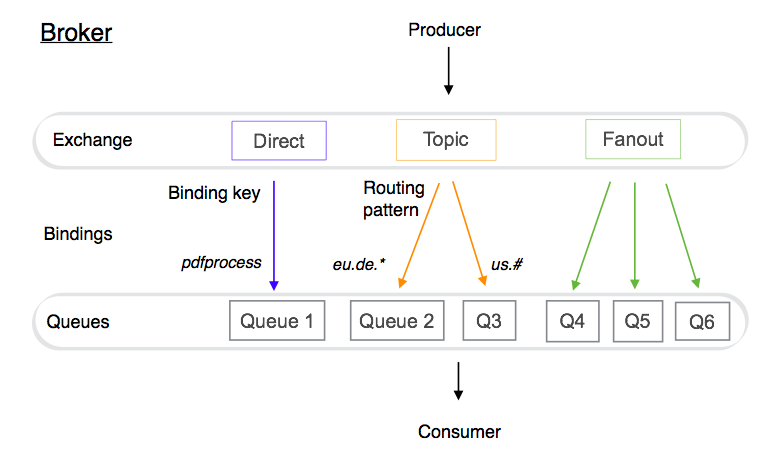
\includegraphics[width=0.9\textwidth]{img/exchanges.png}
\caption{Различия exchanges}
\label{fig6}
\end{figure}

\section{Отличия RabbitMQ и Kafka по гарантии доставке сообщений?}
\section{Области памяти стек и куча}

\begin{figure}[h!]
\centering
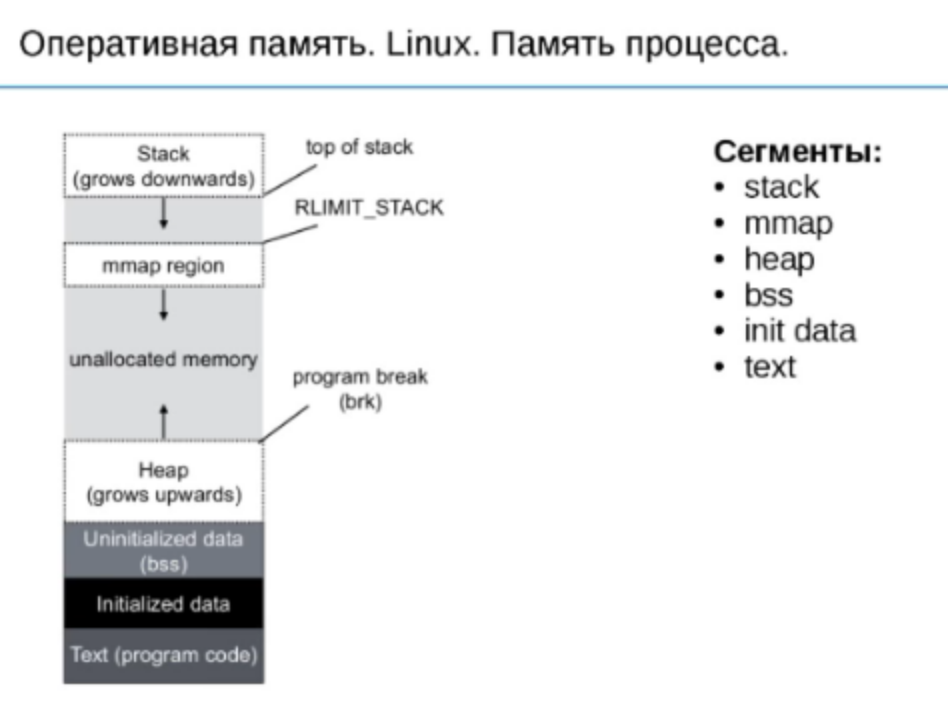
\includegraphics[width=0.8\textwidth]{img/memory.png}
\caption{Memory}
\label{memory}
\end{figure}

\subsection{Стек}

Стек — это область оперативной памяти, которая создаётся для каждого потока. Он работает в порядке LIFO (Last In, First Out),  то есть последний добавленный в стек кусок памяти будет первым в очереди на вывод из стека. Каждый раз, когда функция объявляет новую переменную, она добавляется в стек, а когда эта переменная пропадает из области видимости (например, когда функция заканчивается), она автоматически удаляется из стека. Когда стековая переменная освобождается, эта область памяти становится доступной для других стековых переменных.

Из-за такой природы стека управление памятью оказывается весьма логичным и простым для выполнения на ЦП; это приводит к высокой скорости, в особенности потому, что время цикла обновления байта стека очень мало, т.е. этот байт скорее всего привязан к кэшу процессора. Тем не менее, у такой строгой формы управления есть и недостатки. Размер стека — это фиксированная величина, и превышение лимита выделенной на стеке памяти приведёт к переполнению стека. Размер задаётся при создании потока, и у каждой переменной есть максимальный размер, зависящий от типа данных. Это позволяет ограничивать размер некоторых переменных (например, целочисленных), и вынуждает заранее объявлять размер более сложных типов данных (например, массивов), поскольку стек не позволит им изменить его. Кроме того, переменные, расположенные на стеке, всегда являются локальными.

В итоге стек позволяет управлять памятью наиболее эффективным образом — но если вам нужно использовать динамические структуры данных или глобальные переменные, то стоит обратить внимание на кучу.

\subsection{Куча}

Куча — это хранилище памяти, также расположенное в ОЗУ, которое допускает динамическое выделение памяти и не работает по принципу стека: это просто склад для ваших переменных. Когда вы выделяете в куче участок памяти для хранения переменной, к ней можно обратиться не только в потоке, но и во всем приложении. Именно так определяются глобальные переменные. По завершении приложения все выделенные участки памяти освобождаются. Размер кучи задаётся при запуске приложения, но, в отличие от стека, он ограничен лишь физически, и это позволяет создавать динамические переменные.

Вы взаимодействуете с кучей посредством ссылок, обычно называемых указателями — это переменные, чьи значения являются адресами других переменных. Создавая указатель, вы указываете на местоположение памяти в куче, что задаёт начальное значение переменной и говорит программе, где получить доступ к этому значению. Из-за динамической природы кучи ЦП не принимает участия в контроле над ней; в языках без сборщика мусора (C, C++) разработчику нужно вручную освобождать участки памяти, которые больше не нужны. Если этого не делать, могут возникнуть утечки и фрагментация памяти, что существенно замедлит работу кучи.

В сравнении со стеком, куча работает медленнее, поскольку переменные разбросаны по памяти, а не сидят на верхушке стека. Некорректное управление памятью в куче приводит к замедлению её работы; тем не менее, это не уменьшает её важности — если вам нужно работать с динамическими или глобальными переменными, пользуйтесь кучей.

\section{Прогрев кешей}

\section{Из каких базовых вещей состоят контейнеры: namespaces, cgroups}
	Все инструменты контейнеризации — будь то Docker, LXC или systemd-nspawn,— основываются на двух подсистемах ядра Linux: namespaces и cgroups. 
	
	\subsection{chroot}
	
	Идеи, лежащие в основе механизма пространств имён, не новы. Ещё в 1979 году в UNIX был добавлен системный вызов chroot() — как раз с целью обеспечить изоляцию и предоставить разработчикам отдельную от основной системы площадку для тестирования. 
	
	Название chroot представляет собой сокращение от change root, что дословно переводится как «изменить корень». С помощью системного вызова chroot() и соответствующей команды можно изменить корневой каталог. Программе, запущенной с изменённым корневым каталогом, будут доступны только файлы, находящиеся в этом каталоге. 
	
	Вершиной этой иерархии является каталог /, он же root. Все остальные каталоги — usr, local, bin и другие, — связаны с ним.

С помощью chroot в систему можно добавить второй корневой каталог, который с точки зрения пользователя ничем не будет отличаться от первого. Файловую систему, в которой присутствует изменённый корневой каталог, можно схематично представить на рис. \ref{3}.

\begin{figure}[h!]
\centering
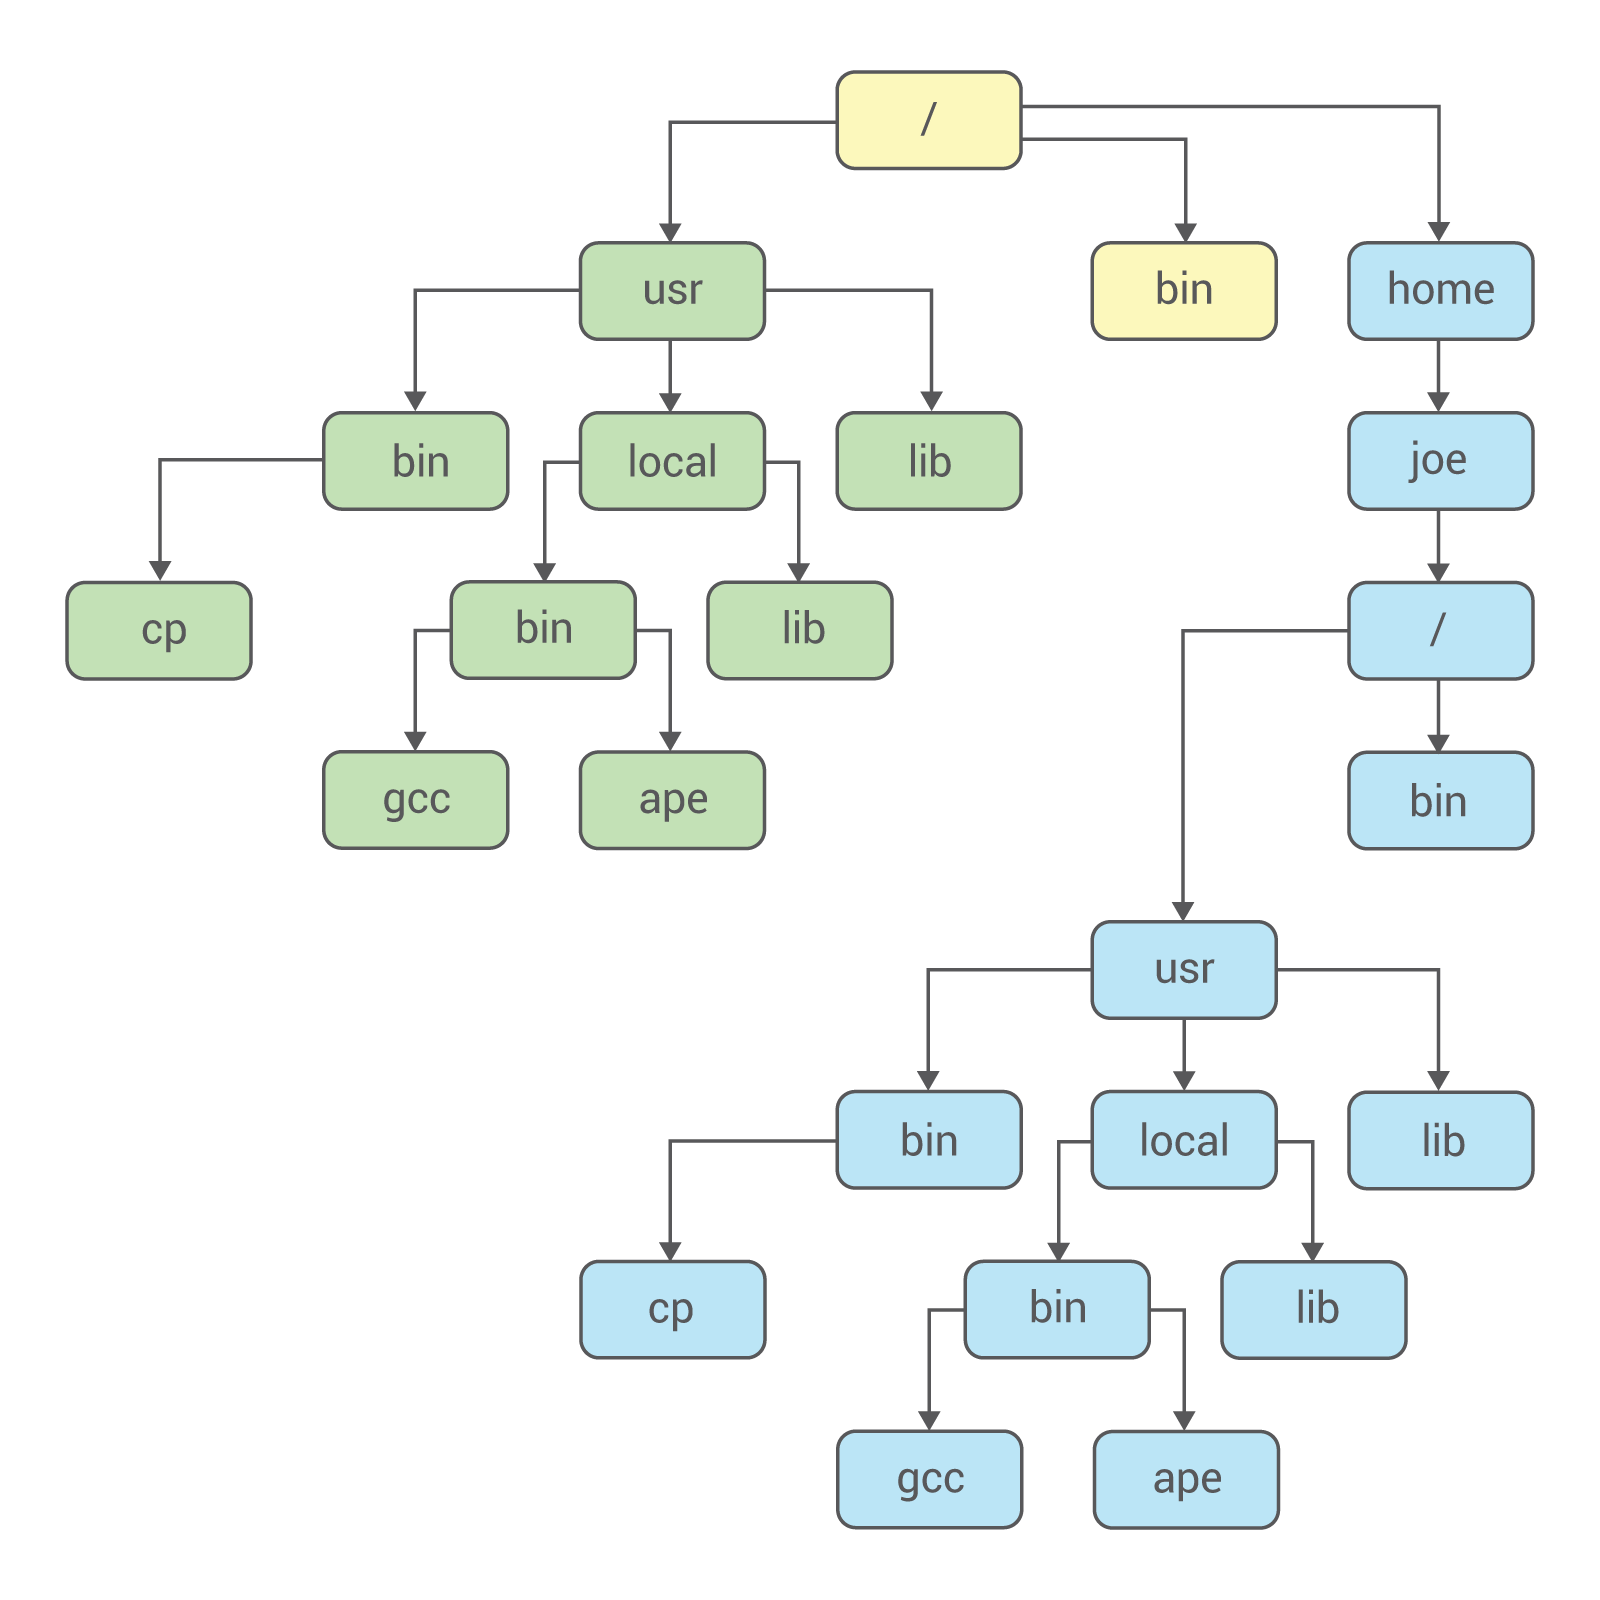
\includegraphics[width=0.9\textwidth]{img/chroot.png}
\caption{Представление файловой системы linux}
\label{fig3}
\end{figure}

\subsection{namespaces}

Пространство имён (англ. namespace) — это механизм ядра Linux, обеспечивающий изоляцию процессов друг от друга. Работа по его реализации была начата в версии ядра 2.4.19. На текущий момент в Linux поддерживается шесть типов пространств имён:

\begin{table}[]
\begin{tabular}{|l|l|}
\hline
Пространство имен & Что изолирует  \\ \hline
PID & PID процессов  \\ \hline
NETWORK & Сетевые устройства, стеки, порты... \\ \hline
USER & ID пользователей и групп \\ \hline
MOUNT & Точки монтирования \\ \hline
IPC & SystemV IPC, очереди сообщений POSIX \\ \hline
UTS & Имя хоста и доменное имя NIS \\ \hline
\end{tabular}
\end{table}

Неймспейсы изолируют друг от другая процессы таким образом, что процессы в одной группе не могут видеть ресурсы другой группы. Например, PID namespace предоставляет уникальные идентификаторы процессов в рамках группы. Внутри одной группы может быть процесс с pid 1 и внутри второй группы тоже может быть процесс с pid 1, хотя это два совершенно разных процесса, которые друг о другие ничего не знают. Притом, все процессы все также имеют уникальные id в рамках ОС. Просто, если смотреть на процессы из группы, то эти id отображаются в другие.

\subsubsection{PID: изоляция PID процессов}

При загрузке в Linux сначала запускается процесс с идентификационным номером (PID) 1. В дереве процессов он является корневым. Он запускает другие процессы и службы. Механизм namespaces позволяет создавать отдельное ответвление дерева процессов с собственным PID 1. Процесс, который создаёт такое ответвление, являются частью основного дерева, но его дочерний процесс уже будет корневым в новом дереве.

Процессы в новом дереве никак не взаимодействуют с родительским процессом и даже не «видят» его. В то же время процессам в основном дереве доступны все процессы дочернего дерева. Наглядно это показано на рис.

\begin{figure}[h!]
\centering
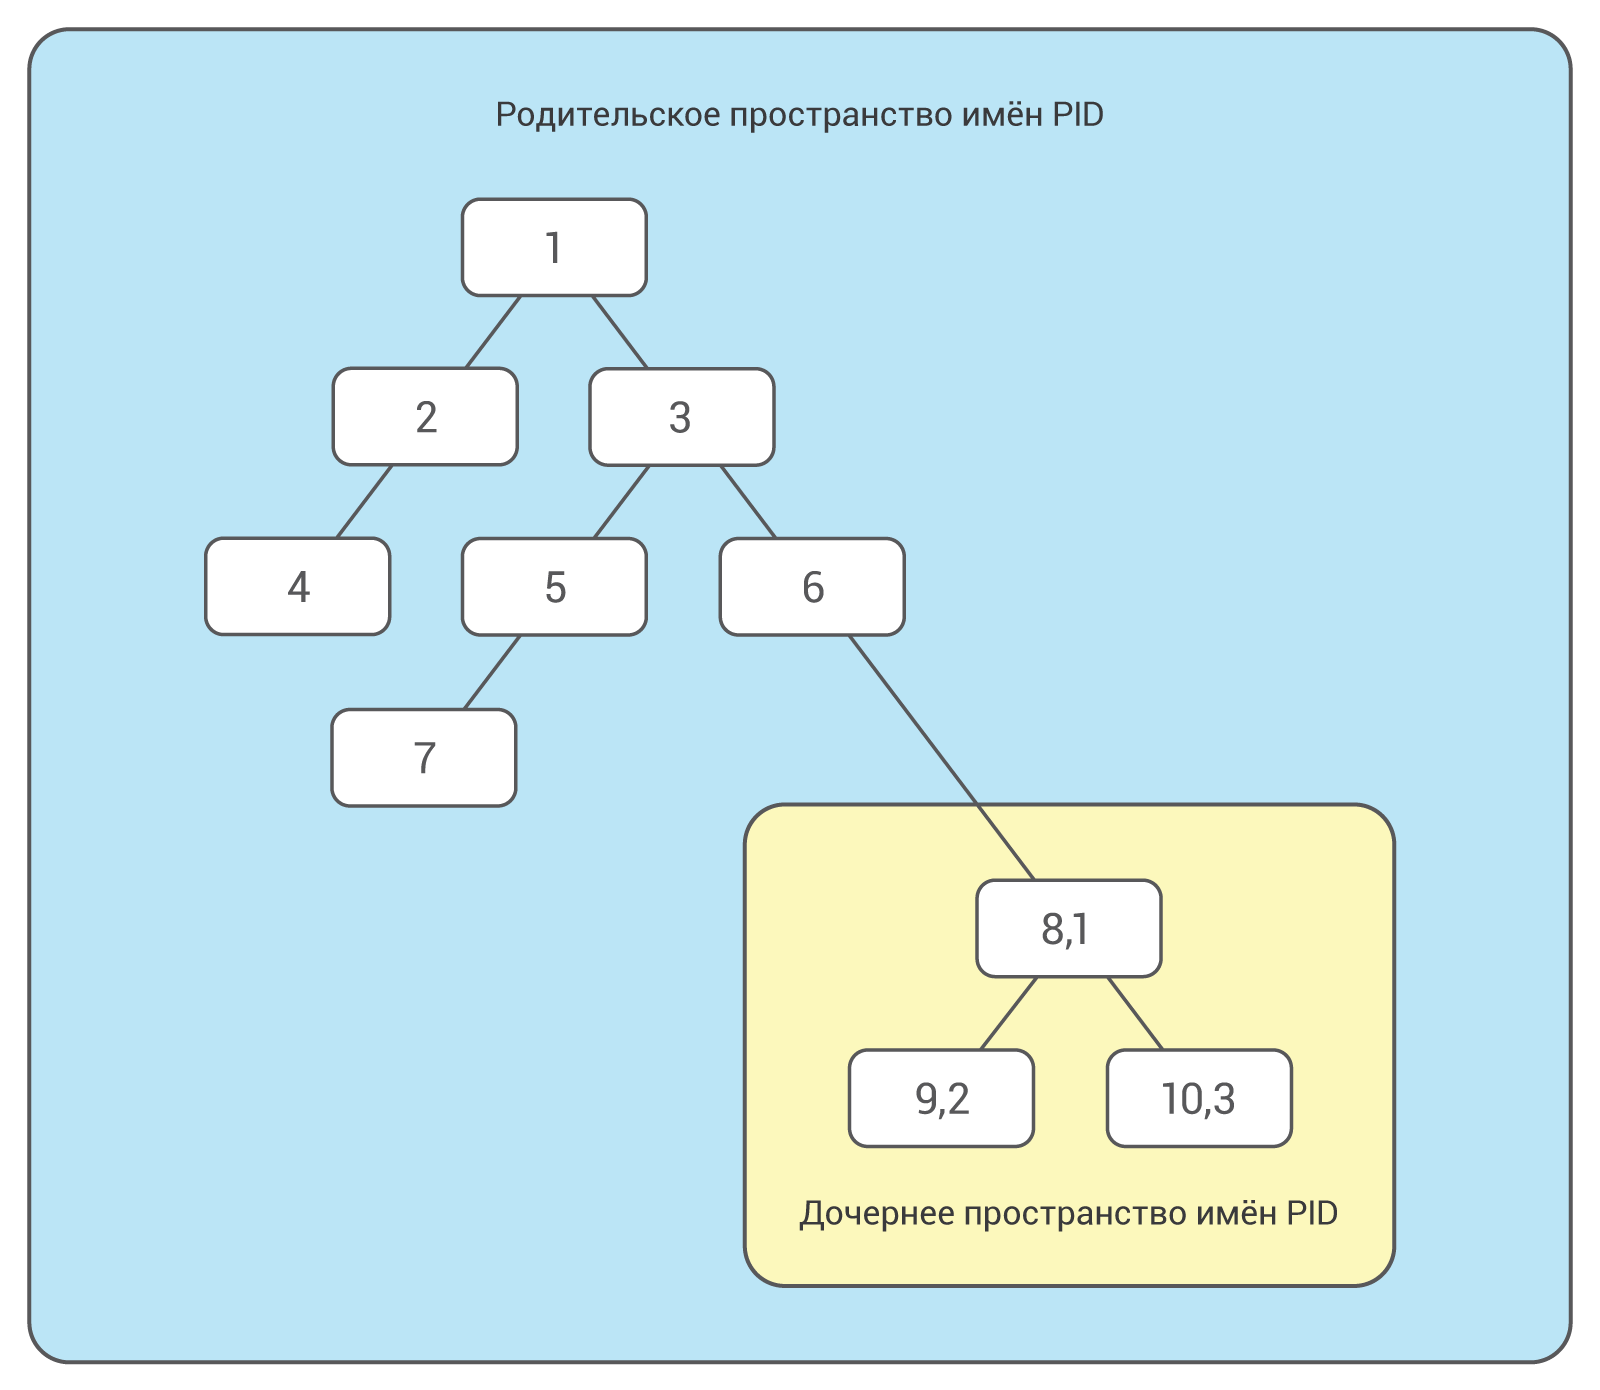
\includegraphics[width=0.9\textwidth]{img/pid.png}
\caption{Представление файловой системы linux}
\label{fig4}
\end{figure}

\subsubsection{NET: изоляция сетей}

Благодаря пространству имён NET мы можем выделять для изолированных процессов собственные сeтевые интерфейсы. Даже loopback-интерфейс для каждого пространства имён будет отдельным.

Сетевые пространства имён можно создавать с помощью системного вызова clone() с флагом CLONE\_NEWNET. 

\subsubsection{MOUNT: изоляция файловой системы}

Об изоляции на уровне файловой системы мы уже упоминали выше, когда разбирали системный вызов chroot (). Мы отметили, что системный вызов chroot() не обеспечивает надёжной изоляции. С помощью же пространств имён MOUNT можно создавать полностью независимые файловые системы, ассоциируемые с различными процессами.

\subsection{cgroups (Control Groups)}

Позволяют организовывать процессы в группы и для каждой группы задавать лимиты. Например, лимиты на использование CPU, объем используемой памяти и дисковый ввод-вывод.

Механизм cgroups состоит из двух составных частей: ядра (cgroup core) и так называемых подсистем. В ядре версии 4.4.0.21 таких подсистем 12:

\begin{itemize}
   \item blkio — устанавливает лимиты на чтение и запись с блочных устройств;
    \item cpuacct — генерирует отчёты об использовании ресурсов процессора;
    \item cpu — обеспечивает доступ процессов в рамках контрольной группы к CPU;
    \item cpuset — распределяет задачи в рамках контрольной группы между процессорными ядрами;
    \item devices — разрешает или блокирует доступ к устройствам;
    \item freezer — приостанавливает и возобновляет выполнение задач в рамках контрольной группы
    \item hugetlb — активирует поддержку больших страниц памяти для контрольных групп;
    \item memory — управляет выделением памяти для групп процессов;
    \item net\_cls — помечает сетевые пакеты специальным тэгом, что позволяет идентифицировать пакеты, порождаемые определённой задачей в рамках контрольной группы;
    \item netprio — используется для динамической установки приоритетов по трафику;
    \item pids — используется для ограничения количества процессов в рамках контрольной группы.
\end{itemize}

Каждая подсистема представляет собой директорию с управляющими файлами, в которых прописываются все настройки.  

\subsection{Отличия namespaces от cgroups}

\textbf{cgroup}: Контрольные группы предоставляют механизм для агрегирования или разбиения наборов задач и всех их будущих детей в иерархические группы со специализированным поведением.
\textbf{namespace}: обертывает глобальный системный ресурс в абстракции, которая заставляет его казаться процессам в пространстве имен, что у них есть свой отдельный экземпляр глобального ресурса.

\textbf{Вкратце}:

     cgroups = ограничивает, сколько вы можете использовать;
     namespaces = пределы того, что вы можете видеть (и, следовательно, использовать)

\section{Времена доступа}

\begin{figure}[h!]
\centering
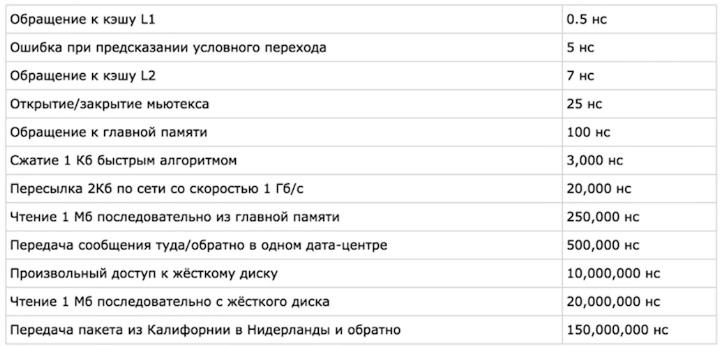
\includegraphics[width=0.8\textwidth]{img/time.png}
\caption{Time}
\label{time}
\end{figure}

\part{Databases}

\chapter{Основные понятия}

\section{Теорема CAP}

Теорема CAP (известная также как теорема Брюера) — эвристическое утверждение о том, что в любой реализации распределённых вычислений возможно обеспечить не более двух из трёх следующих свойств:
\begin{itemize}

 \item согласованность данных (англ. consistency) — во всех вычислительных узлах в один момент времени данные не противоречат друг другу;
\item доступность (англ. availability) — любой запрос к распределённой системе завершается корректным откликом, однако без гарантии, что ответы всех узлов системы совпадают;
\item устойчивость к разделению (англ. partition tolerance) — расщепление распределённой системы на несколько изолированных секций не приводит к некорректности отклика от каждой из секций.

\end{itemize}

\section{Чем отличается транзакция от запроса в контексте БД}
Транзакция - это несколько последовательных запросов в БД, если хотя бы одна из них завершается, то вся транзакция отменяется (rolling back).

\section{Что такое ACID}
\section{Есть ли транзакция в Redis?}

\chapter{Масштабируемость}

\section{Что такое согласованность данных?}

\section{Алгоритмы разрешения конфликтов при репликации}
\subsection{Quorum}
\subsection{Векторные часы}

\section{Шардирование}
\section{Оптимистичные блокировки и пессимистичные?}

\section{Реляционная теория}
\subsection{Что такое транзитивная завивсимость?}
\subsection{Нормальные формы?}
\begin{enumerate}
    \item 1ая;
    \item 2ая;
    \item 3ая;
    \item Бойса-Кодда;
    \item 4ая;
    \item Доменная форма;
    \item 5ая;
    \item 6ая;
\end{enumerate}
\subsection{Ограничение целостности базы данных?}


\chapter{PostgreSQL}

\section{Архитектура posgres}
\subsection{Внутренние компоненты}
\subsection{Что такое autovacuum?}
\section{Что такое план запроса?}

\section{Индексы в postgres}

\subsection{Типы индексов}
\subsubsection{b-tree}
\subsubsection{hash}
\subsubsection{gin}
\subsubsection{gist}
\subsubsection{sp-gist}
\subsubsection{brin}

\section{Что такое include индексы?}
\section{Как посмотреть индексы для таблицы?}
\section{Всегда ли postgres использует индексы?}

\section{Типы данных Redis}

\subsection{Строки (strings)}
Базовый тип данных Redis. Строки в Redis бинарно-безопасны, могут использоваться так же как числа, ограничены размером 512 Мб.
\subsection{Списки (lists)}
Классические списки строк, упорядоченные в порядке вставки, которая возможна как со стороны головы, так и со стороны хвоста списка. Максимальное количество элементов - 232 - 1.
\subsection{Множества (sets)}    
Множества строк в математическом понимании: не упорядочены, поддерживают операции вставки, проверки вхождения элемента, пересечения и разницы множеств. Максимальное количество элементов - 232 - 1.
\subsection{Хеш-таблицы (hashes)}    
Классические хеш-таблицы или ассоциативные массивы. Максимальное количество пар «ключ-значение» - 232 - 1.
\subsection{Упорядоченные множества (sorted sets)}
Упорядоченное множество отличается от обычного тем, что его элементы упорядочены по особому параметру «score».

\end{document}